\documentclass[11pt]{article}
\usepackage[right=1in,left=1in,top=1in,bottom=1in]{geometry}
\usepackage{hyperref}
\hypersetup{colorlinks, citecolor=blue, filecolor=blue, linkcolor=blue, urlcolor=blue}
\usepackage{graphicx}
\usepackage{url}
\usepackage{adjustbox}
\usepackage[round]{natbib}
\usepackage{amsmath,amsthm}
\usepackage{engord}
\usepackage{float}
\usepackage{subfig}
\usepackage{pdflscape}
\usepackage{booktabs}
\usepackage{endnotes}
\usepackage{pgfplots}
\usepackage{subfig}
\pgfplotsset{compat=1.14}
\usepackage{longtable}
\pgfplotsset{every axis label/.append style={font=\tiny}}
\usepackage[labelsep=period]{caption} %% This switches "Table 1: Title" to "Table 1. Title"
\usepackage{authblk}
\usepackage{amssymb} %% Necessary, just for the \checkmark command  in tables.
\usepackage{multirow} %% Necessary if we are doing tables in LaTeX

\usepackage{xr}


\newtheorem{assumption}{Assumption}
\newtheorem{definition}{Definition}
\newtheorem{proposition}{Proposition}
\newtheorem{corollary}{Corollary}
\newtheorem{lemma}{Lemma}
\newtheorem{remark}{Remark}
\newtheorem{example}{Example}
\newtheorem{theorem}{Theorem}

\usepackage{setspace}
\doublespacing

\usepackage{sectsty}
\sectionfont{\large}
\subsectionfont{\normalsize}
\subsubsectionfont{\normalsize}

\newcommand{\specialcell}[2][c]{\begin{tabular}[#1]{@{}l@{}}#2\end{tabular}}

%%%%%%%%%%%%%%%%%%%%%%%%%%%%%%%%%%%%%%%%%%%%%%%%%%%%%%%%%%%%%

\title{ \vspace*{-2.5cm} \hspace*{-0.5cm}Offline Store Expansion and Platform Consolidation: Evidence from major cities in China \footnote{
The preliminary version was entitled "Property brokerage, Partial monopoly and Housing market" and was presented at The 1st Summer Meeting in Urban Economics, China. We are grateful for the comments and suggestions made at the meeting. The code to replicate the paper can be accessed at \href{https://github.com/sergiozxy/RealEstateBrokerage}{https://github.com/sergiozxy/RealEstateBrokerage} The authors gratefully acknowledge financial support from the Fundamental Research Funds for the Central Universities of Sichuan University (2019hhf-08; SKSYL201812; 2018jj-01) and National Natural Science Foundation of China (71773081). % We gratefully thank for Hanying Liu from Sichuan University and Chongyu Wang from Florida State University for insightful feedback.
}}


\date{ \vspace*{0.5cm} \today}

%%%%%%%%%%%%%%%%%%%%%%%%%%%%%%%%%%%%%%%%%%%%%%%%%%%%%%%%%%%%%

\begin{document}


\author[1]{Guoying Deng}
\author[2]{Xuyuan Zhang \thanks{Email Address: \href{mailto:zxuyuan@umich.edu}{zxuyuan@umich.edu}}}
\affil[1]{School of Economics, Sichuan University, China}
\affil[2]{Department of Economics, University of Michigan, United States}

\bgroup
\let\footnoterule\relax

\begin{singlespace}
\maketitle

% Police brutality, law enforcement, and crime: Evidence from Chicago
\begin{abstract}
    \noindent This study examines the impact of offline store expansion by Lianjia, China's leading real estate brokerage, within the framework of platform consolidation. By analyzing micro-level transactions of second-hand houses in ten major Chinese cities from 2016 to 2022, the research investigates how the transaction patterns of traditional brokerages, characterized by the strategic clustering of offline stores, transition towards online consolidation, thereby facilitating the development of an extensive franchise network. Utilizing a regression discontinuity (RD) design, the study quantifies the optimal influence radius of offline stores on housing transactions. Incorporating this optimal influence radius, the study further empirically estimates the effects of real estate brokerage's offline store expansion and online platform consolidation on transaction properties. This analysis leverages the exogenous shock of Lianjia's market entry, identifying a significant increase in transaction revenues before the COVID-19 pandemic. However, this effect diminishes during the pandemic due to remote work and restrictive policies implemented by the Chinese government. The study also examines the online platform consolidation effect by analyzing the period in 2018 when Lianjia revised and improved its Agent Cooperation Network (ACN). 
    
    \textbf{The results indicate that this strategy significantly boosts revenues and also suggest that the offline store's effect is majorly focused on people's transaction behaviors but the online platform's effect can be more insightful to provide a more efficient transaction process. } % this need to be revised.

    This study provides valuable insights into the synergy between offline store expansion and online platform development, elucidating future trajectories in the evolving real estate brokerage market and analogous sectors.
  \end{abstract}
  
  \textbf{Keyword}: Marketing Strategy, Digital Platforms, Platform Consolidation, Real Estate Brokerage
  
  \textbf{JEL} Classification Codes: D4, L1, L8, R3
\end{singlespace}
\thispagestyle{empty}

\clearpage
\egroup
\setcounter{page}{1}

%% Temporary tool to track how this paper is structured. Feel free to comment in or out. 
% \tableofcontents
% \bigskip

%%%%%%%%%%%%%%%%%%%%%%%%%%%%%%%%%%%%%%%%%%%%%%%%%%%%%%%%%%%%%
%%%%\section{Introduction\label{sec:introduction}}

\section{Introduction \label{sec:introduction}}

\noindent

Understanding housing markets is crucial due to their significant impact on household finance, as housing is typically the largest component of a household's portfolio. The illiquidity of housing creates a strong link between housing and labor markets, and transaction costs are critical for buyers and sellers in the real estate market. Real estate brokers play a vital role in reducing these costs, providing essential market information, negotiation support, and legal assistance to ensure smoother and more efficient transactions. With the improvement of China's legal system in the real estate market, the brokerage market is expanding and becoming more prosperous. Especially in the context of China's burgeoning real estate market, brokerage firms are assuming an increasingly important role in facilitating the communications between buyers and sellers \citep{glaeser_real_2017}. Given the heterogeneous and "thin" nature of real estate goods \citep{HAN2015813}, the expertise and local market knowledge of real estate brokers have become indispensable in navigating the complex real estate landscape.

China's real estate market possesses distinct features characterized by the prominence of offline stores, setting it apart from the markets in other developed countries. Compared to the United States, where the Multiple Listing Service (MLS) provides comprehensive and reliable information online, facilitating transactions in a market where houses are typically situated far apart, the role of offline real estate stores is minimized. In contrast, China's real estate market is predominantly offline-based, with online listings serving mainly as references. Face-to-face interactions remain crucial for transactions. Additionally, the Chinese government imposes stringent restrictions on the online listing prices, leading to a reluctance among sellers to list their properties online. This regulatory environment allows real estate brokerages to sometimes post misleading prices to attract potential buyers, subsequently offering private information about other properties. In Singapore, the real estate market is heavily influenced by government-coordinated prices and evaluation companies' suggested prices. Conversely, in China, sellers have more freedom to set arbitrary listing prices. It is common practice for Chinese sellers to list their properties at higher prices, anticipating that buyers will negotiate and feel incentivized by securing a perceived better deal.

Even though the Chinese real estate brokerage market has traditionally been characterized by intense competition among offline stores, the advent of online platforms has dramatically reshaped the dynamics of real estate transactions. Brokerage consolidation, a process where larger firms absorb smaller ones into a unified platform, is emerging as a transformative trend, redefining how properties are bought and sold across China. Lianjia, the largest real estate brokerage in China, has revolutionized real estate transactions through the establishment of the Beke platform. This platform enables rapid expansion by integrating offline stores on a large scale while leveraging the advantages of resource sharing. However, prior to 2018, the platform Beke primarily focused on facilitating listings from Lianjia's offline stores and aimed to attract buyers from the market. However, in 2014, Beke established a new strategy named Agent Cooperate Network (ACN), which integrates and shares the content across its multiple subsidiaries to realize multiple revenue models simultaneously.\footnote{The ACN model disaggregates the transaction process into specialized tasks handled by individual agents or stores. These tasks include seller-side activities such as sourcing sellers, maintaining property listings, commission negotiations, and buyer-side activities like client acquisition, property-client matching, transaction facilitation, and financial services assistance.} Moreover, in 2018, Lianjia decided to enhance its Agent Cooperation Network (ACN) strategy by incorporating smaller brokerages into its network and launching franchise stores under the brand name Deyou, along with other smaller formats. This strategic move aimed to increase network effects and further consolidate the platform, thereby enhancing market power and operational efficiency.

Through the success of the platform consolidation, Lianjia transforms internal competition within the system into overall system competitiveness, thereby enhancing the brand's reputation and market influence. More importantly, this strategic allows Lianjia to cooperate with other previously competitors by consolidating resources. According to Beke's IPO prospectus, Lianjia held approximately a 20.8\% market share in China's second-hand housing market in 2020. However, data from AutoNavi Map indicates that Lianjia's share of stores nationwide was less than 5\%. Notably, in major cities such as Beijing and Shanghai, Lianjia's market share exceeded 45\% and 30\%, respectively, based on data from the local Housing and Urban-Rural Development Committees. Despite this, Lianjia's offline store share in these cities was less than 25\% in Beijing and 10\% in Shanghai, highlighting a significant discrepancy between market presence and physical store distribution. This remarkable market penetration underscores the efficacy of Beke's integrated platform and ACN model in dominating the real estate brokerage landscape. The Figure \ref{fig:precise_proportion_contraction} illustrates the distribution of Lianjia's offline stores across China. The data reveals a significant concentration of these stores in first-tier cities, indicating a pronounced regional disparity. Lianjia's offline store presence is notably uneven, with a high density in major urban centers and sparse distribution in other regions, reflecting strategic market positioning and possibly underlying economic and demographic factors influencing store locations. 

% \subsection{Why Offline Operation is Critical In Real Estate Transaction} \label{subsec:why_offline_is_critical}


 % https://36kr.com/p/2450037897386121#:~:text=%E6%A0%B9%E6%8D%AE%E5%8C%97%E4%BA%AC%E4%BD%8F%E5%BB%BA%E5%A7%94%E6%95%B0%E6%8D%AE,%E6%80%BB%E7%AD%BE%E7%BA%A6%E5%A5%97%E6%95%B0%E7%9A%8439%25%E3%80%82

% https://36kr.com/p/2268329112035080

\begin{figure}
  \centering
  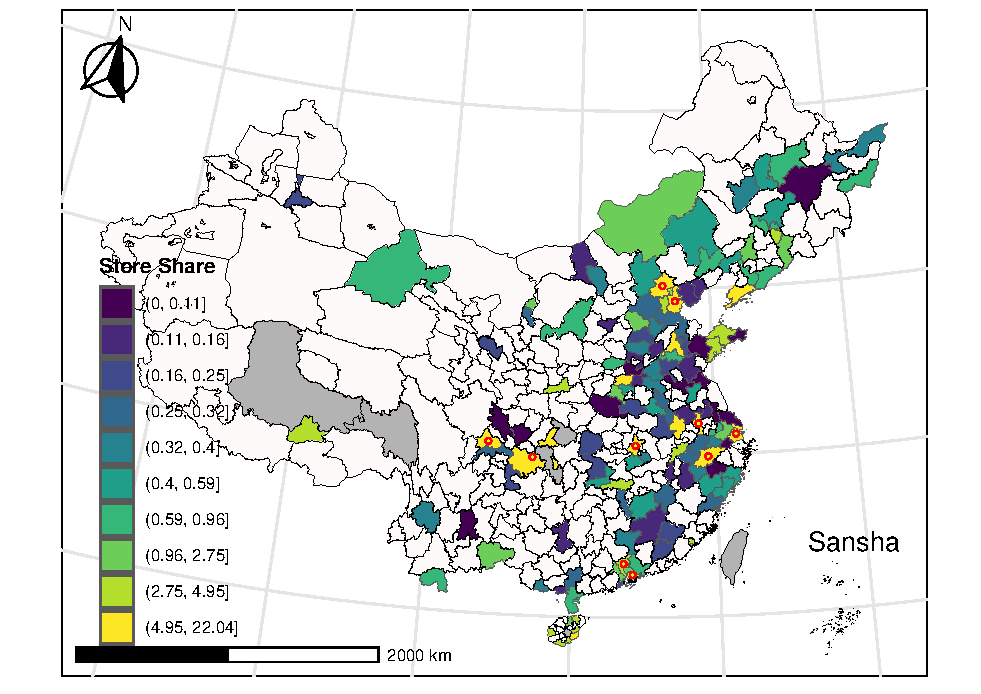
\includegraphics[width=0.7\textwidth]{../figures/distribution_of_cities_share.pdf}
  \caption{Distribution of Lianjia's stores' percentage across China}
  \label{fig:precise_proportion_contraction}
  Note: This plot displays the percentage of Lianjia's offline stores in each city relative to the total number of brokerages in that city, based on data from AutoNavi Map. Gray areas indicate invalid information, while white areas denote cities without any Lianjia stores. Additionally, Sansha city is featured in the bottom right corner of the graph.
\end{figure}

Additionally, in the China's real estate market, brokerages still operate on a bilateral agency model, where sellers need to choose the agency that can help them sell their home in the fastest time and for the highest price possible for the transaction. However, due to the asymmetric information inherent in the real estate market, sellers face challenges in effectively informing and matching with potential buyers. In a perfectly competitive market, sellers would be indifferent in their choice of real estate agents. Nonetheless, as the market trends toward increased monopolization, sellers confront a dichotomous decision: engage a larger brokerage firm, which, despite higher fees, offers the potential for expedited transactions, or opt for a smaller brokerage with lower fees but potentially less efficient transaction facilitation.

While sellers might consider a co-listing strategy—listing their property with multiple brokerages—this approach is suboptimal for several reasons within China's real estate market. Despite previous literature, such as \citep{RePEc:kap:jrefec:v:67:y:2023:i:3:d:10.1007_s11146-021-09858-w}, indicating that the co-listing can be beneficial for clients under multiple-listing service. Specifically in China's real estate market, firstly, the exclusivity of contracts between sellers and agents often precludes the adoption of a co-listing strategy. Secondly, although sellers can list their properties with multiple brokerages, smaller agencies frequently lack a sufficiently broad client base, limiting their effectiveness in selling homes. Thirdly, engaging multiple brokers simultaneously can lead to reduced incentives among agents, as they perceive competition for the same property, diminishing their proactive efforts. Finally, while service cost variations between agencies are acknowledged, these costs are minor compared to the property's value and are more closely related to the risks associated with holding a financial asset. Consequently, risk-averse sellers are inclined to choose an agency that provides a guaranteed level of service. 

Given the dual nature of online promotion and offline transactions in the real estate brokerage industry, the quality of offline services is crucial for influencing client decisions. This principle underpins Lianjia's strategy of establishing numerous stores within targeted communities. By opening a wide range of stores in various neighborhoods and adopting a downstream consolidation model through platform design, the brokerage effectively attracts sellers to list their properties and buyers through its extensive platform resources. This strategy not only enhances transaction volume but also increases income derived from these transactions.

In this paper, we empirically estimate the effects of offline store clustering and online platform consolidation in China's second-hand real estate market. Utilizing micro-level transaction data, we construct our research sample by aggregating information at the neighborhood level. We employ a regression discontinuity (RD) design to identify the optimal influential radius of offline stores on neighborhood transactions, finding that this radius corresponds to a brokerage's five-minute walk service distance. Subsequently, we apply a difference-in-difference (DID) estimation method to evaluate the exogenous impact of Lianjia's market entry on local segments. This exogenous effect captures the clustering impact of offline real estate brokerage stores. Our results indicate that Lianjia's offline stores significantly enhance transaction revenues, although this effect diminishes during and after the COVID-19 period.

To assess the consolidation effect of the online platform, we treat the year Lianjia implemented the platform consolidation strategy as an exogenous shock to the market. The platform consolidation strategy is majorly based on the Agent Cooperation Network (ACN) framework of Lianjia and attracting various franchise stores to join the network. Our findings reveal that this strategy substantially boosts revenues and alters consumer behaviors, particularly in the number of house tours facilitated by the brokerage. 










% WE ARE WORKING ON THIS

These results underscore the necessity for a synergistic evolution of online and offline strategies in the real estate brokerage market. Furthermore, we find that the online consolidation effect is and the effect is 

Lastly, the network effect has cross stores according to the IPO prospectus, in year 2021, Lianjia is expected to achive approximately 76\% of cross stores transactions.


















% Accodring to 招股书,链家在2021的成交是cross store占比76\%

Our research has several implications. Firstly, it indicates that with the advent of new technologies, the online consolidation effect is becoming increasingly important for real estate companies. This shift underscores the need for firms to enhance their digital strategies to remain competitive. Secondly, our findings have broader significance for other industries where online consolidation can potentially replace traditional offline clustering. For example, in the retail sector, online marketplaces such as Alibaba in China have significantly outpaced physical stores by consolidating various vendors into a single, accessible platform.

By examining these dynamics, our research contributes to a deeper understanding of the evolving landscape of real estate brokerage in China. It provides valuable insights for policymakers and industry stakeholders aiming to enhance market efficiency and competitiveness. As the online consolidation effect continues to grow, our findings highlight the importance of adapting to this trend and evolving strategies accordingly. Specifically, transitioning from a bilateral brokerage model to a model where buyer and seller agencies are separated could be crucial for sustaining a competitive advantage in the real estate brokerage market. This strategic shift entails leveraging online platforms to integrate services and enhance transaction efficiency, thereby benefiting both consumers and firms. By disentangling the roles of buyer and seller agents, the market can reduce conflicts of interest, increase transparency, and improve overall market efficiency. This alignment with economic principles of specialization and efficiency further underscores the potential for significant gains in consumer welfare and firm profitability.

The remainder of the paper proceeds as follows. Section \ref{sec:literature_review} reviews the literature that is related to our research. Section \ref{sec:data} describes the study background and statistical summary. Section \ref{sec:mechanism_design} presents the main result of our finding. Finally, Section \ref{sec:conclusion} contains the discussion and concludes.

\section{Literature Review} \label{sec:literature_review}

The literature on the real estate market, particularly the role of real estate brokerages, is extensive and informative, starting with the foundational work of \citet{Rosen_hedonic} who introduced the hedonic pricing model. This model breaks down property prices by analyzing internal and external factors. However, it's worth noting that this model does not adequately account for market asymmetries and information disparities, leading to potential inaccuracies in pricing. A fundamental study by \citep{Akerlof_1970} highlights the significant impact of asymmetric information on market dynamics, using the market for used cars as an example. Here, the prevalence of low-quality goods, known as 'lemons', often leads to market inefficiencies, a problem that is mirrored in the real estate sector. The challenge of asymmetric information in real markets was further emphasized by \citet{grossman_impossibility_1980}, who questioned the feasibility of the effective market assumption, particularly under conditions of information disparity.

Subsequent studies have expanded on these foundational theories, exploring dynamics specific to real estate pricing and strategic behavior. \citet{550a6ccf-cde2-3dd1-979f-1a8db2b8ceb9} documents that apart from price competition in the market, there is a lot of market inefficiency that stems from non-price competition, which suggests that as the degree of competition in the market increases, the market becomes progressively less efficient, indicating that the entry dividend begins to fall and aggregate social welfare begins to decline. Moreover, \citet{hendel_relative_2009} analyzes two types of listings in the second-hand housing market and finds that For-Sale-By-Owner type of platforms are less effective in terms of time and probability of sale while operating better compared to listing homes for sale as a broker. In addition, \citet{bailey_economic_2018} uses data from the social media site Facebook to show that social interactions can influence people's economic decisions. Their results show that people who have friends who are geographically distant in real life and who have a hunch that house prices are about to rise are more likely to buy a house than rent one. Other relevant areas of research include \citep{SIRMANS1991207, NIEUWERBURGH_information, salz_intermediation_2022}.

The strategic behavior of real estate brokerages has been documented to leverage informational advantages. \citet{AGARWAL2019715} confirms that brokerages, as market intermediaries, possess nuanced knowledge of market conditions, enabling them to negotiate discounts effectively. Furthermore, \citet{HAN2015813} discusses the varying bargaining power of brokerages across unidirectional and bidirectional markets, influencing their operational strategies. This is corroborated by evidence suggesting that properties listed with lower commission rates not only sell less frequently but also take longer to sell \citep{10.1257/app.20160214}. The advent of online platforms has significantly altered the landscape of real estate transactions. \citet{ZUMPANO2003134} notes that while the duration of property searches has not changed markedly, the scope of searches has broadened to encompass more online listings. Moreover, \citet{ZHANG2021101104} associates the rise of online platforms with a reduction in existing home prices and an increase in sales volumes, a dynamic influenced by factors such as new home prices and household demographics. However, a detailed analysis of the impact of the presence of these platforms on market performance of offline stores remains scant.

Moreover, the overall market influence of real estate intermediaries is multifaceted. Utilizing a model predicated on perfect competition, \citet{williams_agency_1998} illustrates that excessive entry of brokers into the market can surpass the optimal allocation, thereby reducing social welfare. This is corroborated by studies indicating that an increase in the number of brokers can depress house prices and shorten transaction cycles \citep{https://doi.org/10.1002/jae.2891}. Additionally, \citet{qu_identifying_2021} highlights the moderating role of broker commissions in disseminating information during transactions, facilitating more efficient home sales. Other related literature includes \citep{doi:10.1080/10527001.2021.2016340, doi:10.1080/10835547.1996.12090852}.

Finally, the concept of the platform as a "two-sided market" or kind of intermediates that connects the buyer side and seller side digitally, \citep{10.1162/154247603322493212, Langley_Leyshon_2017}. Despite the significant attention given to online platforms, there is a lack of systematic analysis on the impact of offline stores of online platforms on market performance or on real estate brokerage. Therefore, this paper aims to fill this gap by examining the influence of offline stores associated with online platforms on the real estate market.

% With respect to the behavior of real estate brokerages, the research conducted by \citep{AGARWAL2019715} substantiates that these entities, acting as intermediaries in market transactions, possess superior knowledge of market dynamics. This informational superiority enables the intermediaries to use their bargaining power to secure discounts in the market. Similarly, \citet{HAN2015813} articulates that brokerages operating in unidirectional and bidirectional markets exhibit different levels of bargaining leverage, leading to different motivational drivers. This mechanism is in line with other research, which shows that properties with lower commission rates have a 5\% less likelihood of being sold and takes 12\% longer to sell \citep{10.1257/app.20160214}.

% Regarding the impact of online platforms on the real estate sector, research by \citep{ZUMPANO2003134} suggests that while the length of time buyers spend searching for properties remains unchanged, the scope of their search expands to include a greater number of online listings. \citet{ZHANG2021101104} show that the introduction of online platforms is associated with reductions in existing home prices and increased sales volumes, effects that are influenced by new home prices and household size. However, a comprehensive analysis of the influence of the physical stores of online platforms on the real estate market is still lacking in the literature. 

% Finally, the impact of real estate intermediaries on the market can be decomposed into several aspects. Using a model based on the assumption of a perfectly competitive market in which an influx of brokers competitively enters the market, \citet{williams_agency_1998} shows that the presence of brokers in the market equilibrium exceeds the optimal number of allocations, thereby causing a reduction in social welfare. Moreover, the results show that neither brokers nor sellers are motivated to deviate from the equilibrium price structure, which coincides with the reservation price set by sellers. Complementary research in another study shows that a significant influx of brokers into the market is correlated with a decrease, rather than an increase, in house prices, along with a gradual decrease in transaction cycles within the market \citep{https://doi.org/10.1002/jae.2891}. Furthermore, the work of \citep{qu_identifying_2021-1} highlights the moderating role of broker commissions on the dissemination of market information during transactions. Their findings suggest that the use of a broker can significantly mitigate the concessions that sellers are forced to make in the transaction process, thereby enhancing their ability to complete a home sale more efficiently.

% Many literature has been conducted to study the real estate market, and the impact of real estate brokerages on the market, beginning with \citet{Rosen_hedonic}, which proposed a hedonic pricing model and decomposed the price by internal and external factors affecting it. However, the hedonic pricing model suffers from market asymmetry and information inequality. The seminal work on the impact of asymmetric information in markets is \citep{Akerlof_1970}, which demonstrated that markets for used cars tend to be dominated by low-quality goods, or 'lemons', leading to market inefficiencies. Furthermore, \citet{grossman_impossibility_1980} further argued that information effective market assumption is hard to hold in reality. Therefore, the real estate market, which is characterized by information asymmetry, is particularly vulnerable to the adverse selection problem. In this context, the role of real estate brokerages is crucial, as they act as intermediaries between buyers and sellers, providing valuable information and facilitating transactions.

% 由于房地产中介行业线上推广线下成交的机制,中介机构在线下门店中的服务性质对于其在客源方的影响具有很高的价值。链家通常选择在每个目标小区的周边开店便是该原理。链家通过在小区周边大范围开店,从而吸引卖方选择该机构进行挂牌,而又通过其广泛的平台客源来吸引市场中的买方从而获得更多的成交数量与成交收入。由于房地产中介行业线上推广线下成交的机制,中介机构在线下门店中的服务性质对于其在客源方的影响具有很高的价值。链家通常选择在每个目标小区的周边开店便是该原理。链家通过在小区周边大范围开店,从而吸引卖方选择该机构进行挂牌,而又通过其广泛的平台客源来吸引市场中的买方从而获得更多的成交数量与成交收入。


\section{Data and Descriptive Evidence \label{sec:data}}

\subsection{Data Collection and Processing} \label{subsec:data_collection}

This study focuses on the housing markets in ten major cities in China, namely Beijing, Shanghai, Chongqing, Tianjin, Shenzhen, Guangzhou, Chengdu, Hangzhou, Wuhan and Nanjing. These cities are not only central to China's economic development, but also reflect the broader trends and characteristics of the country's real estate dynamics. Spanning from 2016 to 2022, the research period encapsulates a pivotal era in China's real estate sector. During the first phase of the study, from 2016 to 2019, the housing markets in these cities experienced a remarkable boom. This period was characterized by significant growth in property prices, supported by robust economic expansion and increased demand in these urban centers. However, the final phase of our study, from 2020 to 2022, paints a contrasting picture. During this period, China's overall economic growth rate has been slower significantly, which has also reflected in a slowdown in the real estate markets of these major cities. In addition, the Chinese government has implemented strict rules in Covid-19 protection, so the real estate agents in these major cities are significantly affected.

The second hand housing transaction data was collected form \href{https://www.ke.com/city/}{beke.com} for ten cities ranging from 2016 to 2022.\footnote{Due to government policy, Lianjia was unable to disclose transaction prices in Beijing, Shenzhen, and Wuhan for the years 2021 and 2022, as well as in Chengdu for 2021. Consequently, we have excluded this period of data for these cities from our analysis.} Initially, we filtered out transaction records exhibiting unusually high prices, identifying them as outliers that could skew the analysis. We then removed records with missing values to maintain the integrity of our dataset. We also removed any records that were listed duplicated. We finally have a data with length 1,778,647 second-hand houses.\footnote{Due to government restrictions, four of these cities did not list the transaction price for each transaction during the study period.} After cleaning the data, we constructed two research samples: one at the individual transaction level and the other at the neighborhood level. The individual transaction sample contains detailed information on each transaction, including the transaction price, transaction date, price concessions, and the number of house tours. The neighborhood-level sample aggregates transaction data at the community level, encompassing variables such as the average transaction price and the average number of house tours. Additionally, we calculated the annual number of house transactions to capture Lianjia's transaction activity within each neighborhood. This data structure enables a comprehensive analysis of the impact of offline stores on housing transactions across both individual and neighborhood dimensions.

To gather additional characteristic information, Point of Interest (POI) data was extracted from the AutoNavi map using a web-scraping Python program.\footnote{AutoNavi, a leading mapping application in China with a user base exceeding 700 million, is renowned for its detailed and accurate POI data as well as precise public transportation information. These features underscore AutoNavi's leadership in the digital mapping sector, highlighting its ability to provide unparalleled navigation accuracy and comprehensive urban mobility solutions. Our extracted AutoNavi dataset includes over one million POIs per city annually.} The extracted POIs were then classified into various categories, as detailed in Table \ref{tab:statistical_district} and Table \ref{tab:statistical_individual} and it primarily represents living facilities, entertainment venues, restaurants, hospitals, and other public amenities. This classification is crucial for understanding the urban infrastructure and amenities available in the vicinity of the analyzed properties.

Each type of POI was matched to our data within a 500-meter radius, a distance typically covered by walking and consistent with urban planning standards for accessible urban design. This radius reflects the immediate urban environment influencing residential desirability and property values, as most of these POIs provide recreational services. Additionally, geo-informational data, including annual GDP data from \citet{zhao_forecasting_2017}, nighttime lights data from \citet{elvidge_annual_2021}, and air pollution data from \citet{doi:10.1021/acs.est.1c05309}, was integrated into our research. The centroid of the neighborhood-level data's polygon was generated, and values from the geo-informational data were extracted. By merging these data sources with our research panel, a comprehensive research sample was constructed.

\subsection{Influential Radius} \label{subsec:Influential_Radius}

The effectiveness of an offline intermediary's influence on its immediate communities is inherently constrained by geographic limitations, with its influence decreasing in proportion to the increase in spatial distance. Moreover, since the offline stores of Lianjia are directly operated by the company, strategic considerations regarding the optimal distance between stores are an integral part of their location planning to mitigate the risks associated with over-concentration of stores that could lead to competitive overlap and service homogenization. Consequently, it is imperative to determine an optimal radius threshold and subsequently assess the diversity of agencies operating within this demarcated zone.

To determine the optimal radius of influence, this research employs a regression discontinuity design (RDD) method on the neighborhood level transaction data to examine the influential radius of offline real estate brokerages. The dependent variable in this analysis is the transaction revenue generated by Lianjia within a given community, while the independent variable is the community's proximity to the nearest Lianjia store. Given that stores are predominantly located within commercial districts, which typically encompass several streets no more than two kilometers in diameter, it is assumed that a requisite number of stores within each district is essential to sustain revenue generation in that community. In addition, Lianjia adopts a 5-minute walking distance (approximately 400 meters) radius policy, which means that no matter how far away customers live, they should be accessible within a 5-minute walk to the nearest Lianjia store. Building on this premise, the study further investigates the existence of an optimal influence radius within shopping districts, defined as the distance radius within which the presence of a Lianjia optimally increases transaction revenues. At the same time, the study also examines the hypothesis that beyond this optimal radius, the impact on transaction revenues diminishes as a result of the strategic store layout decisions implemented by Lianjia.

\begin{figure}[ht]
    \centering
    \subfloat[RD plot with first order polynomial]{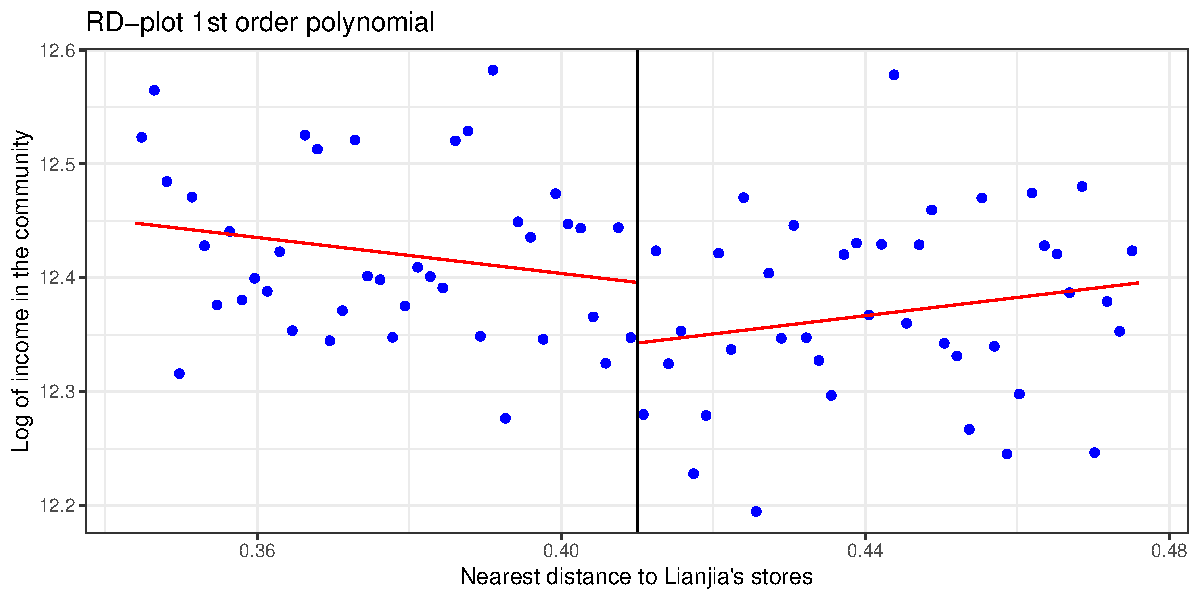
\includegraphics[width=0.5\textwidth]{../figures/RD_Plot_1st_Order.pdf}\label{fig:RD_Plot_1st_Order}}
    \hfill % Adds horizontal space between figures
    \subfloat[RD plot with second order polynomial]{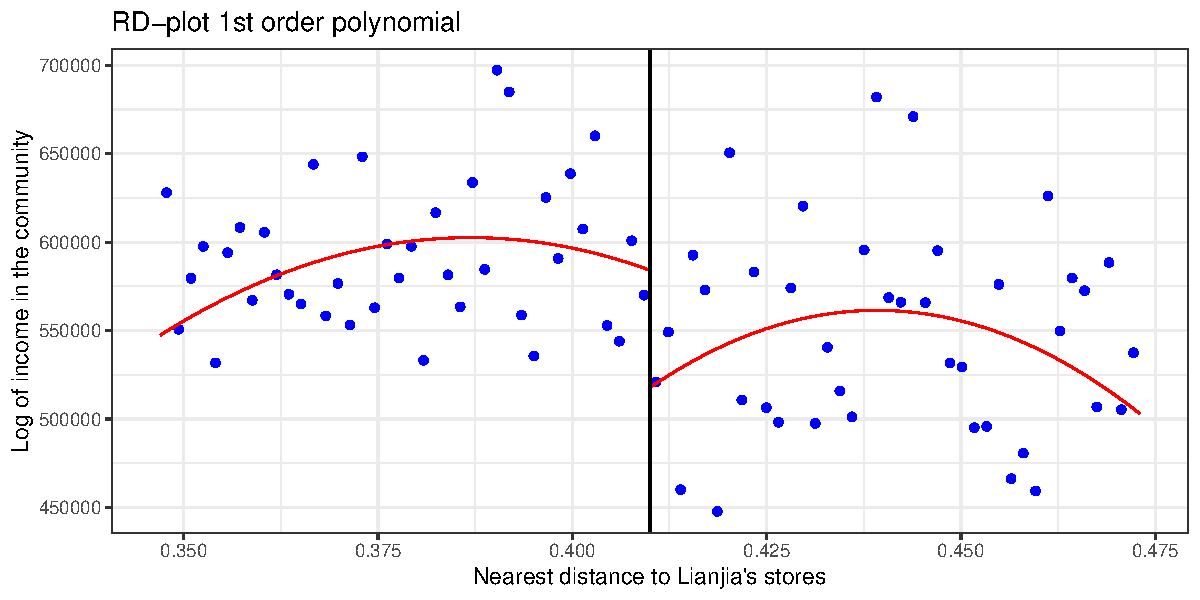
\includegraphics[width=0.5\textwidth]{../figures/RD_Plot_2nd_Order.pdf}\label{fig:RD_Plot_2nd_Order}}
    \hfill % Adds horizontal space between figures
    \subfloat[RD plot with third order polynomial]{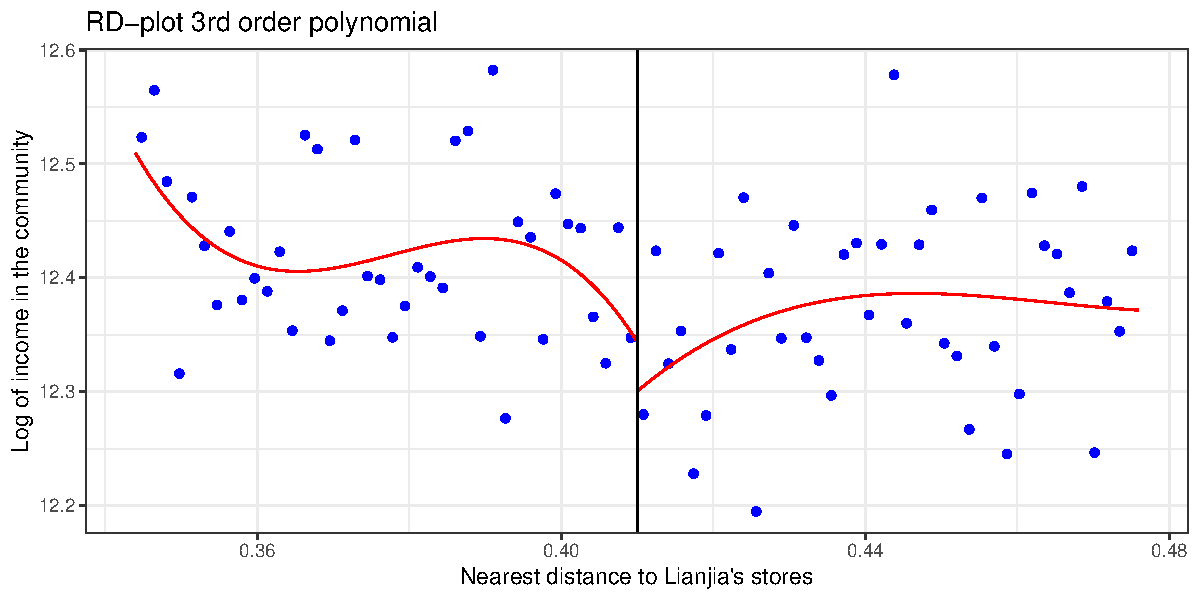
\includegraphics[width=0.5\textwidth]{../figures/RD_Plot_3rd_Order.pdf}\label{fig:RD_Plot_3rd_Order}}
    \caption{RD design}
    \label{fig:RD_design}
\end{figure}

% latex table generated in R 4.2.0 by xtable 1.8-4 package
% Mon Jul  8 21:12:27 2024
\begin{table}[ht]
\centering
\begin{tabular}{lllllllr}
  \hline
Method & Kernel & Estimate & SE & Z & PValue & Bandwidth & EffectiveObs \\ 
  \hline
mserd & uniform & -48903 & 21529 & -2.27 & 0.0231 & 0.0504 & 24269 \\ 
  mserd & triangular & -61304 & 20887 & -2.94 & 0.00333 & 0.063 & 30532 \\ 
  cerrd & uniform & -56899 & 28636 & -1.99 & 0.0469 & 0.0273 & 13166 \\ 
  cerrd & triangular & -59561 & 27943 & -2.13 & 0.033 & 0.0341 & 16392 \\ 
   \hline
\end{tabular}
\caption{RD Estimates with Different Bandwidth Selection Methods and Kernels} 
\label{tab:rd_bandwidth_kernel_results}
\end{table}



From Figure \ref{fig:RD_design} we can see that there is indeed discontinuity in 410 meters of communities to the nearest Lianjia's store, which is pretty close to the lianjia's 5-minute walk distance policy. The observed decline in the Lianjia's influence is marked and suggests a pronounced reduction in its impact on the system overall within our study sample. This phenomenon can be attributed to the implementation of the Lianjia's proximity to customers policy, which is evidenced at the data level. Table \ref{tab:rd_bandwidth_kernel_results} considers different kernel and bandwidth choices, and the results are consistent with the 410 meters radius. The only non-significance is the CER-optimal bandwidth selector with triangular kernel, which is because the selected bandwidth is too small to capture the discontinuity. The results are robust to different bandwidth and kernel choices, which suggests that the 410 meters is the optimal radius for Lianjia's offline stores.

To make the robust check we conducted Donut Hole test by excluding observations close to the cutoff and estimating the effect with the remaining data. The results are shown in Appendix and the result shows that the discontinuity still exists and this provides evidence against a model misspecification. Furthermore, we carry out the density test by \citep{MCCRARY2008698}. The result shows that the p-value is greater than 0.1 (p value equals 0.101), which suggests the result is not due to manipulation of polygons. Finally, we carry out placebo tests which are reported in Appendix, which shows that our result is robust. Specifically, Table \ref{tab:placebo_test_results} shows that the discontinuity does not exist in the placebo test, which suggests that our result is not due to the manipulation of the data. Table \ref{tab:movement_cutoff} shows that other cutoffs do not have the same effect as the 410 meters cutoff, which suggests that the 410 meters is the optimal radius for Lianjia's offline stores.

\subsection{Statistical Summary} \label{subsec:Statistical_Summary}

After constructing our optimal radius, we recalcualte the number of lianjia and other brokerages' stores within this radius. To check the robustness of the data, we divide our data to those with lianjia and those without lianjia and to check whether lianjia's offline stores have influential effect on the transaction effect in the community. We can see that for income, house tour number and the are all significantly different in those communities with or without lianjia. In addition, we find that the other brokerages also have the same tendency that they typically open stores with the same strategy as Lianjia, which suggests that Lianjia does not have the market power to exclude competent companies from entering the market, and it also suggests that the market is not monopolized by Lianjia. We plot the relationship between the number of other brokerages's stores and the number of lianjia's stores and the figure is shown in Figure \ref{fig:same_distribution}.

From Table \ref{tab:statistical_district} we can see that the in our metro areas, the neighborhoods with lianjia within the influential radius tends to have higher number of sales, and the final transaction price is also \textyen 910,000 higher than those neighborhoods without lianjia. Moreover, the number of other stores within the influential distance is also signnificantly more than 7.3, which also aligns with our previous intuition that the market is not monopolized by Lianjia. This significance difference suggests that if we treat our sample as a cross sectional data and estimate the result with static model without considering the individual fixed effect, we may get a biased result. Besides, our model may suffer from endogeneity issue, since the number of lianjia's stores may be endogenous to the transaction price and the number of stores. 

\begin{table}[htb!]
    \centering
    \begin{tiny}
    \caption{Statistical Summary for the Neighborhoods-Data with Lianjia and without Lianjia}
    \begin{tabular}{llllll}
\toprule
Name & Mean without lianjia & SD without lianjia & Mean with lianjia & SD with lianjia & Difference \\
\midrule
\multicolumn{6}{l}{\textbf{Panel 1: }Transaction property} \\
income & 44.44 & 73.85 & 77.68 & 117.3 & -33.24 (-76.638***) \\
lead\_times & 13.59 & 14.56 & 17.09 & 17.50 & -3.501 (-49.823***) \\
price\_concession & -0.0367 & 0.0318 & -0.0351 & 0.0294 & -0.00200 (-12.088***) \\
\multicolumn{6}{l}{\textbf{Panel 2: }brokerage property} \\
density & 0 & 0 & 0.206 & 0.166 & -0.206 (-384.429***) \\
broker\_410 & 5.362 & 6.871 & 12.66 & 8.410 & -7.300 (-217.614***) \\
watching\_people & 17.61 & 29.11 & 20.29 & 29.40 & -2.682 (-21.214***) \\
end\_price & 260.5 & 254.9 & 351.9 & 292.1 & -91.48 (-76.662***) \\
non\_online\_effect & 0.195 & 0.396 & 0.233 & 0.423 & -0.0380 (-21.384***) \\
watched\_times & 1121 & 1827 & 1233 & 1969 & -112.4 (-13.636***) \\
nego\_times & 4.769 & 7.686 & 5.683 & 10.78 & -0.914 (-22.178***) \\
nego\_period & 150.5 & 187.5 & 166.6 & 239.1 & -16.06 (-17.075***) \\
\multicolumn{6}{l}{\textbf{Panel 3: }hedonic information property} \\
jiadian & 1.489 & 3.566 & 1.942 & 4.365 & -0.453 (-26.004***) \\
kind & 8.665 & 6.229 & 11.76 & 6.081 & -3.097 (-116.630***) \\
hotel & 3.211 & 5.287 & 5.428 & 6.315 & -2.217 (-87.264***) \\
shop\_mall & 4.554 & 7.539 & 6.698 & 8.489 & -2.144 (-61.405***) \\
museum & 0.617 & 1.533 & 1.023 & 1.869 & -0.406 (-54.395***) \\
old & 0.894 & 1.628 & 1.339 & 1.950 & -0.446 (-56.870***) \\
ktv & 5.179 & 7.853 & 7.305 & 7.759 & -2.126 (-63.096***) \\
mid & 2.059 & 2.329 & 3.368 & 2.853 & -1.309 (-115.077***) \\
prim & 2.812 & 2.846 & 4.343 & 3.205 & -1.531 (-116.172***) \\
west\_food & 3.880 & 7.709 & 7.317 & 10.02 & -3.437 (-87.756***) \\
super & 3.155 & 3.374 & 4.499 & 3.686 & -1.344 (-87.586***) \\
sub & 0.683 & 0.945 & 1.111 & 1.099 & -0.429 (-96.038***) \\
park & 3.422 & 4.575 & 4.569 & 3.944 & -1.147 (-62.708***) \\
\multicolumn{6}{l}{\textbf{Panel 4: }house property} \\
area & 90.82 & 48.57 & 84.97 & 39.15 & 5.845 (31.050***) \\
bedroom & 2.338 & 0.816 & 2.202 & 0.730 & 0.136 (40.958***) \\
toilet & 1.306 & 0.579 & 1.246 & 0.455 & 0.0600 (26.915***) \\
house\_age & 18.08 & 11.68 & 20.73 & 11.77 & -2.651 (-52.316***) \\
floor\_level & 1.854 & 0.975 & 1.933 & 0.931 & -0.0790 (-19.324***) \\
green\_ratio & 0.309 & 0.237 & 0.300 & 0.107 & 0.00900 (12.288***) \\
total\_building & 26.88 & 56.66 & 20.51 & 50.54 & 6.371 (27.653***) \\
total\_floor\_number & 12.75 & 8.454 & 12.97 & 8.485 & -0.221 (-6.035***) \\
living\_room & 1.445 & 0.504 & 1.341 & 0.492 & 0.104 (48.345***) \\
elevator\_ratio & 0.453 & 0.413 & 0.408 & 0.279 & 0.0450 (30.475***) \\
kitchen & 0.983 & 0.150 & 0.983 & 0.125 & 0 (-0.459) \\
floor\_ratio & 4.942 & 329.1 & 2.702 & 9.385 & 2.240 (2.367**) \\
\multicolumn{6}{l}{\textbf{Panel 5: }regional property} \\
total\_resident & 995.8 & 1079 & 901.8 & 956.5 & 93.97 (21.484***) \\
pm25 & 44.08 & 13.29 & 45.74 & 13.89 & -1.664 (-28.266***) \\
pop & 15506 & 16336 & 24634 & 18866 & -9100 (-118.769***) \\
light & 32.62 & 13.59 & 38.41 & 11.92 & -5.782 (-105.485***) \\
\bottomrule
\end{tabular}

    \label{tab:statistical_district}

    Note that the code book of the variables can be seen in the Appendix \ref{tab:codebook}
    \end{tiny}
\end{table}

\begin{table}[htb!]
  \centering
  \begin{tiny}
  \caption{Statistical Summary for the Individual-Data with Lianjia and without Lianjia}
  \begin{tabular}{llllll}
\toprule
Name & Mean without lianjia & SD without lianjia & Mean with lianjia & SD with lianjia & Difference \\
\midrule
\multicolumn{6}{l}{\textbf{Panel 1: }Transaction property} \\
income & 0.493 & 0.656 & 0.797 & 0.974 & -0.304 (-226.763***) \\
lead\_times & 16.83 & 26.13 & 20.47 & 31.23 & -3.648 (-80.341***) \\
price\_concession & -2.791 & 2.984 & -2.703 & 2.776 & -0.0890 (-19.908***) \\
\multicolumn{6}{l}{\textbf{Panel 2: }brokerage property} \\
density & 0 & 0 & 0.235 & 0.182 & -0.235 (-1.1e+03***) \\
broker\_410 & 4.620 & 6.135 & 11.39 & 7.999 & -6.765 (-596.183***) \\
watching\_people & 18.49 & 59.53 & 22.13 & 49.02 & -3.647 (-44.332***) \\
end\_price & 229.8 & 197.1 & 305.3 & 237.0 & -75.50 (-219.538***) \\
non\_online\_effect & 0.232 & 0.422 & 0.238 & 0.426 & -0.00600 (-9.241***) \\
watched\_times & 1128 & 2226 & 1235 & 2387 & -106.8 (-29.718***) \\
nego\_times & 6.275 & 15.16 & 6.636 & 17.65 & -0.361 (-13.948***) \\
nego\_period & 139.0 & 197.5 & 141.8 & 225.4 & -2.840 (-8.544***) \\
\multicolumn{6}{l}{\textbf{Panel 3: }hedonic information property} \\
jiadian & 0.299 & 1.492 & 0.379 & 1.683 & -0.0800 (-32.152***) \\
kind & 2.253 & 2.136 & 3.347 & 2.421 & -1.094 (-305.752***) \\
hotel & 0.586 & 1.413 & 1.022 & 1.762 & -0.436 (-172.389***) \\
shop\_mall & 0.896 & 2.355 & 1.463 & 3.000 & -0.567 (-132.449***) \\
museum & 0.103 & 0.492 & 0.146 & 0.526 & -0.0430 (-53.977***) \\
old & 0.194 & 0.582 & 0.273 & 0.690 & -0.0790 (-78.187***) \\
ktv & 1.021 & 2.439 & 1.611 & 2.726 & -0.590 (-145.734***) \\
mid & 0.468 & 0.851 & 0.753 & 1.079 & -0.285 (-184.969***) \\
prim & 0.666 & 0.996 & 1.034 & 1.146 & -0.368 (-218.091***) \\
west\_food & 0.716 & 1.942 & 1.423 & 2.640 & -0.707 (-190.757***) \\
super & 2.515 & 2.959 & 3.748 & 3.356 & -1.233 (-248.593***) \\
sub & 0.143 & 0.365 & 0.247 & 0.461 & -0.104 (-158.165***) \\
park & 0.671 & 1.319 & 0.916 & 1.292 & -0.245 (-121.784***) \\
\multicolumn{6}{l}{\textbf{Panel 4: }house property} \\
area & 86.14 & 40.03 & 81.62 & 36.37 & 4.518 (77.381***) \\
bedroom & 2.285 & 0.873 & 2.145 & 0.854 & 0.140 (105.281***) \\
toilet & 1.261 & 0.554 & 1.222 & 0.481 & 0.0400 (50.222***) \\
house\_age & 15.47 & 10.88 & 18.36 & 11.45 & -2.888 (-166.420***) \\
floor\_level & 1.851 & 0.977 & 1.890 & 0.959 & -0.0390 (-25.910***) \\
green\_ratio & 0.325 & 0.168 & 0.319 & 0.0942 & 0.00600 (31.022***) \\
total\_building & 34.11 & 64.21 & 30.05 & 67.64 & 4.061 (39.620***) \\
total\_floor\_number & 15.81 & 9.744 & 15.47 & 9.637 & 0.348 (23.296***) \\
living\_room & 1.436 & 0.574 & 1.319 & 0.575 & 0.117 (131.401***) \\
elevator\_ratio & 0.430 & 0.376 & 0.390 & 0.250 & 0.0400 (84.381***) \\
kitchen & 0.988 & 0.144 & 0.988 & 0.136 & 0 (0.385) \\
floor\_ratio & 2.923 & 124.3 & 2.738 & 6.971 & 0.184 (1.555) \\
\multicolumn{6}{l}{\textbf{Panel 5: }regional property} \\
total\_resident & 1899 & 1750 & 1903 & 1666 & -4.785 (-1.824*) \\
pm25 & 45.49 & 13.47 & 48.01 & 14.35 & -2.519 (-116.310***) \\
pop & 12369 & 14407 & 19596 & 17151 & -7200 (-289.518***) \\
light & 31.41 & 12.98 & 36.56 & 11.92 & -5.155 (-270.639***) \\
\bottomrule
\end{tabular}

  \label{tab:statistical_individual}

  Note that the code book of the variables can be seen in the Appendix \ref{tab:codebook}
  \end{tiny}  
\end{table}

\begin{figure}
    \centering
    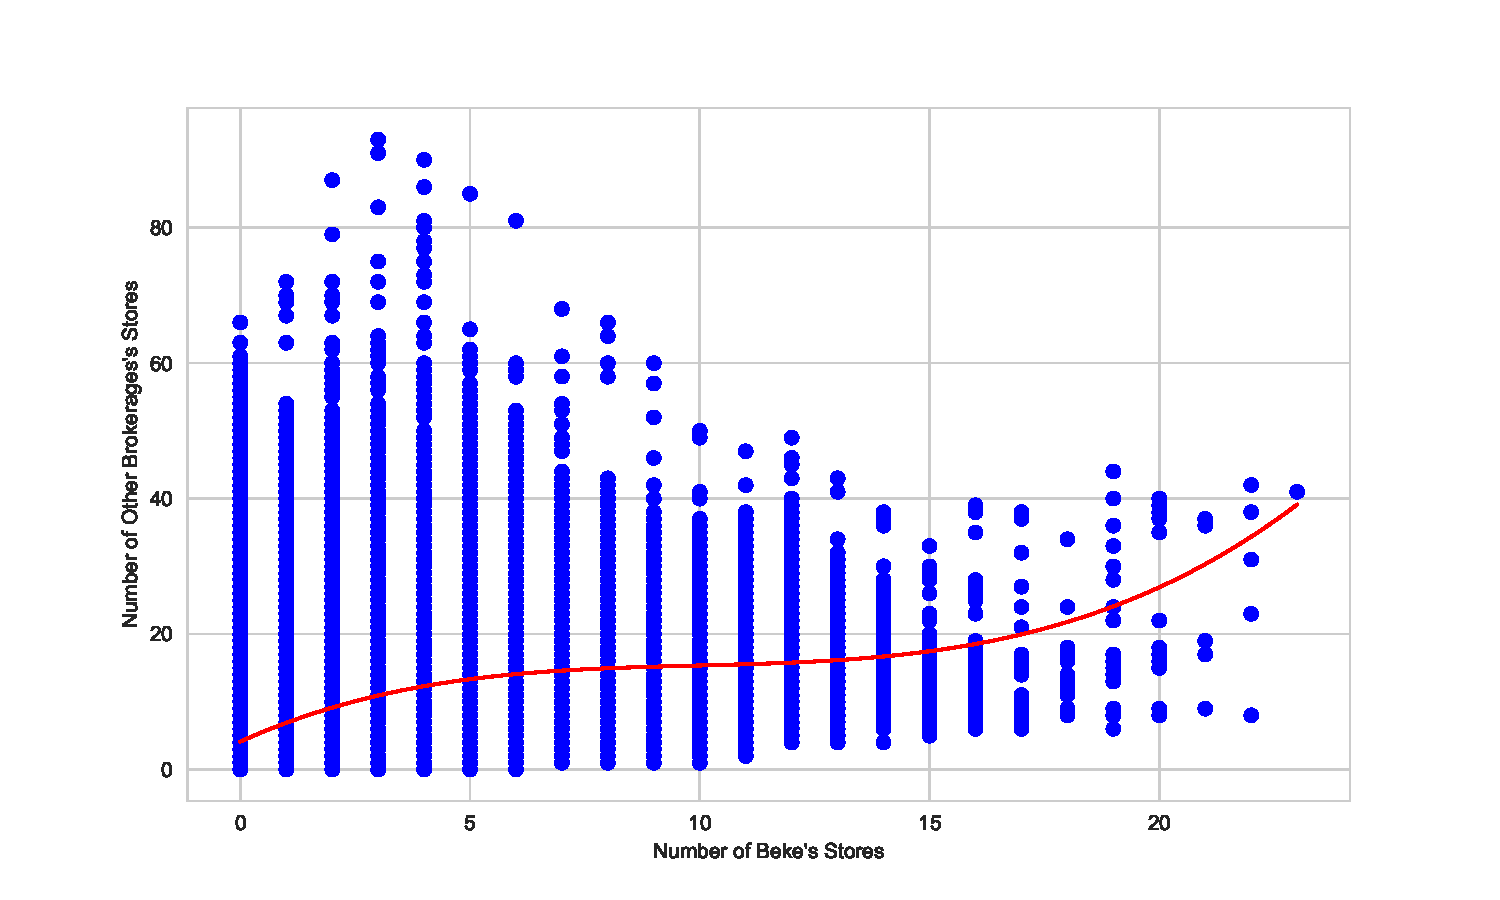
\includegraphics[width=0.7\textwidth]{../figures/scatter_plot_with_two_brokerages.pdf}
    \caption{Tendency between two types of brokerages}
    \label{fig:same_distribution}
    Note: the x-axis is the number of lianjia's stores and the y-axis is the number of other brokerages' stores. The fit is a cubic polynomial fit.
\end{figure}


\subsection{Stylized Fact} \label{subsec:stylized_fact}

In our analysis, we focus on several dependent variables: \emph{the natural logarithm of lianjia's income}, \emph{the natural logarithm of home tours}, \emph{the natural logarithm of transaction period} and \emph{the price concession}. To quantify Lianjia's impact, we begin by establishing a key stylized fact, which we develop a Density-Based Index (DBI) index to capture the Lianjia's offline stores' influential ratio. The index is to measure the effects of Lianjia's operations and its continuous expansion. The definition of this index is informed by the results of an influential radius test, which helps us capture the spatial extent of Lianjia's influence on local real estate markets. This approach allows for a more nuanced understanding of how Lianjia's presence affects key market variables. The DBI is calculated as follows:

\begin{equation*}
  density_{it} = \frac{lianjia_{it}}{total_{it}},
\end{equation*}

where $lianjia_{it}$ represents the number of Lianjia's stores within a 410-meter radius and $total_{it}$ denotes the total number of real estate brokerages' stores within the same radius. The choice of this index is grounded in an effort to address potential reverse causality issues. Specifically, Lianjia and other brokerages often strategically place their stores in highly desirable locations, which typically also results high transaction volumes. This could potentially will caused our estimation biased if we were to simply count the number of Lianjia's stores. To control for this issue, we employ a comparative metric: the ratio of Lianjia brokerages to the total number of real estate brokerages within the radius. This ratio helps mitigate the bias that may arise from the strategic location choices of Lianjia, offering a clearer measure of its market influence relative to competitors. This approach aligns with the principles of spatial competition theory, as articulated in \citep{hotelling_stability_1929, daspremont_hotellings_1979} in competition model. Such a comparative metric not only provides a more accurate reflection of Lianjia's market penetration but also adheres to economic modeling standards by accounting for competitive dynamics in the sector.

To capture the individual fixed effect and other time-invariant unobservable influential factors, a multi-way fixed effect model is proposed. The model is specified as follows: 

\begin{equation}
  Y_{it} = \beta_0 + \beta_1 density_{it} + \bf{\alpha} \bf{X}_{it} + \tau_{it} + \mu_i + \epsilon_{it}, \label{eq:multi-way-fe}
\end{equation}

where $Y_{it}$ is the three main dependent variables, including $\log(\text{income})$, price concession, and $\log(\text{number of house tours})$, $density_{it}$ is the DBI, $\bf{X}_{it}$ is a set of control variables, including brokerage\_control L\_hedonic\_control, transaction\_control and region\_control, while $\tau_{it}$ is the time dummy variable interacting with the fixed effect of the business area, $\mu_i$ is the individual fixed effect and $\epsilon_{it}$ is the error term. The standard errors are clustered at the each community level. The results are shown in Table \ref{tab:stylized_fact}.

\begin{table}[htb!]
    \centering
    \begin{scriptsize}
    {
\def\sym#1{\ifmmode^{#1}\else\(^{#1}\)\fi}
\begin{tabular}{l*{3}{c}}
\toprule
            &\multicolumn{1}{c}{(1)}&\multicolumn{1}{c}{(2)}&\multicolumn{1}{c}{(3)}\\
            &\multicolumn{1}{c}{log(income)}&\multicolumn{1}{c}{price concession}&\multicolumn{1}{c}{log(lead times)}\\
\midrule
density     &      0.0718\sym{***}&   -0.000542         &      0.0397\sym{**} \\
            &    (0.0203)         &  (0.000775)         &    (0.0156)         \\
\addlinespace
Other Brokerage Num  &     0.00100         &   0.0000171         &   -0.000348         \\
            &   (0.00116)         & (0.0000425)         &  (0.000781)         \\
\addlinespace
log(watch people)&      0.0662\sym{***}&     0.00189\sym{***}&       0.333\sym{***}\\
            &   (0.00378)         &  (0.000154)         &   (0.00432)         \\
\addlinespace
ln(Price)&       0.920\sym{***}&      0.0707\sym{***}&       0.240\sym{***}\\
            &    (0.0298)         &   (0.00226)         &    (0.0232)         \\
\addlinespace
log(watch time)&      0.0309\sym{***}&   -0.000237\sym{**} &      0.0318\sym{***}\\
            &   (0.00244)         & (0.0000953)         &   (0.00206)         \\
\addlinespace
log(nego changes)&      0.0240\sym{***}&     0.00202\sym{***}&       0.135\sym{***}\\
            &   (0.00635)         &  (0.000247)         &   (0.00703)         \\
\addlinespace
log(negotiation period)&      0.0598\sym{***}&    -0.00189\sym{***}&       0.131\sym{***}\\
            &   (0.00350)         &  (0.000169)         &   (0.00395)         \\
\midrule
\(N\)       &      134648         &      132301         &      134648         \\
R-squared   &       0.886         &       0.610         &       0.918         \\
\bottomrule
\multicolumn{4}{l}{\footnotesize Standard errors in parentheses}\\
\multicolumn{4}{l}{\footnotesize \sym{*} \(p<0.1\), \sym{**} \(p<0.05\), \sym{***} \(p<0.01\)}\\
\end{tabular}
}

    \caption{The DBI influence to the lianjia's transaction}

    Note: we omit all the control variables in the regression model, and detailed descriptions can be seen from Table \ref{tab:statistical_district} and Table \ref{tab:statistical_individual}.
    \label{tab:stylized_fact}
    \end{scriptsize}
\end{table}

In column 1 and 2, we estimated the model using the neighborhood-level data and in column 3 and 4, we estiamted the model using the individual-level data, respectively. The results show that the share of Linajia's offline stores in total brokerage plays a significant role in the real estate market, especially in terms of revenue and lead time, but not in terms of price concession and transaction period. Specifically, a 1\% increase in a Lianjia's DBI within an area correlates with a 7\% increase in income, as indicated in column 1. Furthermore, this increased DBI also leads to a 4\% increase in the number of home tours in the column 2, underscoring the Lianjia's increased visibility and potential for customer engagement. In contrast, the analysis shows no significant effect of DBI on price concessions and transaction time. This finding suggests that while a larger market share increases revenues and the number of house tours, it may not be beneficial for mathcing the buyers and sellers. The broader implications point to the strategic advantage of density or market share in driving business performance metrics, except for pricing strategies, which appear to be unaffected by changes in market share.

Within the temporal scope of our investigation, the dataset encapsulates two distinct epochs: a phase characterized by surging housing prices and the subsequent period marked by the COVID-19 pandemic. These intervals were further complicated by regulatory measures enacted by the Chinese government, significantly altering the operational dynamics and influence of brokerages within the housing market. Acknowledging these temporal shifts necessitates a nuanced analysis of the brokerage effect across different stages of the study period to ensure the robustness of our findings. To address this, we adopt a dynamic analytical approach, dissecting the period into annual segments. This granularity is achieved by constructing seven unique variables, each representing the interaction between brokerage density and the respective $density_{it} * year_{it}$. Our methodology employs a multi-way fixed effects model, as detailed in Equation \eqref{eq:dynamic}, which facilitates a comprehensive examination of temporal variations in the brokerage's market impact.

In the construction of our regression model, we deliberately omit the first period to avoid multicollinearity problem, treating it as a baseline for comparison. This strategic choice allows us to refine our proxy variable—the product of Lianjia's Dealership Balance Index (DBI) and annual dummies—as a more precise measure of Lianjia's local market power. Besides, to control for potential self correlation problem, we also included lagged one period dependent variables in the model.  Other settings are the same with the previous model \eqref{eq:multi-way-fe} and the result is reported in Table \ref{tab:Dynamic}: 

\begin{equation}
    Y_{it} = \beta_0 + \rho Y_{it-1} + \sum_{i=2}^7 density_{it} * year_{it} + \bf{\alpha} \bf{X}_{it} + \tau_{it} + \mu_i + \epsilon_{it}. \label{eq:dynamic}
\end{equation}

\begin{table}[H]
  \begin{center}
    \begin{scriptsize}
    \caption{Dynamic Regression Results}
    \label{tab:Dynamic}
    {
\def\sym#1{\ifmmode^{#1}\else\(^{#1}\)\fi}
\begin{tabular}{l*{4}{c}}
\toprule
            &\multicolumn{1}{c}{(1)}&\multicolumn{1}{c}{(2)}&\multicolumn{1}{c}{(3)}&\multicolumn{1}{c}{(4)}\\
            &\multicolumn{1}{c}{log(income)}&\multicolumn{1}{c}{log(lead times)}&\multicolumn{1}{c}{log(negotiation period)}&\multicolumn{1}{c}{price concession}\\
\midrule
year2 $\times$ density&       0.209\sym{***}&      0.0404         &      0.0639\sym{**} &   -0.000194         \\
            &    (0.0345)         &    (0.0248)         &    (0.0282)         &  (0.000592)         \\
\addlinespace
year3 $\times$ density&       0.160\sym{***}&      0.0894\sym{***}&     0.00336         &    0.000978\sym{*}  \\
            &    (0.0302)         &    (0.0226)         &    (0.0209)         &  (0.000551)         \\
\addlinespace
year4 $\times$ density&      0.0623\sym{**} &      0.0463\sym{**} &     -0.0168         &    0.000528         \\
            &    (0.0298)         &    (0.0221)         &    (0.0249)         &  (0.000501)         \\
\addlinespace
year5 $\times$ density&      0.0868\sym{***}&      0.0485\sym{**} &     -0.0581\sym{**} &    0.000331         \\
            &    (0.0307)         &    (0.0214)         &    (0.0278)         &  (0.000459)         \\
\addlinespace
year6 $\times$ density&      -0.182\sym{***}&    -0.00849         &     -0.0363         &    -0.00247\sym{***}\\
            &    (0.0540)         &    (0.0357)         &    (0.0359)         &  (0.000868)         \\
\addlinespace
year7 $\times$ density&      -0.133\sym{**} &      0.0395         &     -0.0346         &    -0.00404\sym{***}\\
            &    (0.0573)         &    (0.0493)         &    (0.0413)         &   (0.00108)         \\
\addlinespace
other brokerage num  &     0.00203\sym{*}  &    0.000597         &   -0.000995         &  0.00000271         \\
            &   (0.00107)         &  (0.000733)         &  (0.000828)         & (0.0000138)         \\
\addlinespace
ln(Price)&       0.931\sym{***}&       0.240\sym{***}&      -0.220\sym{***}&      0.0130\sym{***}\\
            &    (0.0300)         &    (0.0232)         &    (0.0210)         &  (0.000550)         \\
\addlinespace
log(watch people)&      0.0680\sym{***}&       0.328\sym{***}&       0.358\sym{***}&    0.000582\sym{***}\\
            &   (0.00377)         &   (0.00427)         &   (0.00266)         & (0.0000376)         \\
\addlinespace
log(watch time)&      0.0301\sym{***}&      0.0327\sym{***}&      0.0386\sym{***}&   -0.000587\sym{***}\\
            &   (0.00242)         &   (0.00202)         &   (0.00188)         & (0.0000296)         \\
\addlinespace
log(nego changes)&      0.0230\sym{***}&       0.133\sym{***}&       0.652\sym{***}&     0.00188\sym{***}\\
            &   (0.00635)         &   (0.00691)         &   (0.00577)         & (0.0000577)         \\
\addlinespace
log(negotiation period)&      0.0579\sym{***}&       0.126\sym{***}&                     &                     \\
            &   (0.00348)         &   (0.00388)         &                     &                     \\
\midrule
\(N\)       &      134648         &      134648         &     1771638         &     1736077         \\
R-squared   &       0.887         &       0.919         &       0.520         &       0.233         \\
\bottomrule
\multicolumn{5}{l}{\footnotesize Standard errors in parentheses}\\
\multicolumn{5}{l}{\footnotesize \sym{*} \(p<0.1\), \sym{**} \(p<0.05\), \sym{***} \(p<0.01\)}\\
\end{tabular}
}


    Note: we omit all the control variables in the regression model, and detailed descriptions can be seen from Table \ref{tab:statistical_district} and Table \ref{tab:statistical_individual}.
    \end{scriptsize}
  \end{center}
\end{table}

The result highlights the dynamic impact of density, encapsulated by Lianjia's DBI, on transaction revenue, house tours, and price concessions over time, especially in response to external factors such as digital transformation and the COVID-19 pandemic. Initially, Lianjia's impact on transaction revenue showed a significant positive trend, peaking in 2018, due to its digital transformation efforts, including the integration of other platform stores into its shared network. However, the momentum slowed in 2020 and 2021, with the impact becoming significantly negative. This period coincided with the outbreak of the COVID-19 pandemic, which severely disrupted Lianjia's revenue streams and business activities due to widespread restrictions, underscoring the vulnerability of real estate transactions to macroeconomic shocks. In terms of home tours, Lianjia's impact remained robustly positive through 2019. This suggests that a strong market presence correlates with increased buyer attention, which translates into more home tours. However, pandemic-related restrictions dampened this effect in later years, highlighting the challenges posed by external constraints on physical real estate activity. For price concessions, we find that the Lianjia's DBI is significantly negatively correlated with the price concessions during pandemic periods. This is due to the fact that most transactions slow down during these periods and people are more likely to wait longer to find a buyer, which would result in fewer price concessions.

To verify the robustness of our results, we calculated the Herfindahl-Hirschman Index (HHI) for each segmented market, defined as $HHI = \sum_{i=1}^N (s_i)^2$ where $s_i$ is the market share of firm $i$ expressed as a percentage. We then estimated the model by dividing the sample into high HHI (greater than 2000) and low HHI (less than 2000) groups. The results, shown in Table \ref{tab:sylized_fact_hetero_hhi}, indicate that Lianjia's offline stores have a more substantial impact on transaction properties in more competitive markets compared to more monopolized ones. This effect arises from two main factors: first, Lianjia's market power is insufficient to exclude other competitors from entering the market, and second, the area may not be attractive to other competitors, resulting in a larger market share for Lianjia. Furthermore, to address the heterogeneity issue, we introduced a dummy variable equal to one if the market already had Lianjia presence before 2016 and estimated the model by separating the sample based on this criterion. The results, presented in Table \ref{tab:sylized_fact_hetero_mature}, demonstrate that the years 2017, 2018, and 2019 have a significant positive impact on Lianjia's revenue in this segmented market. Another interesting phenomenon observed is that the number of house tours is significant for the years 2018 and 2019 in the lower maturity group, whereas in the higher maturity group, the number of house tours becomes significant in 2020. These findings indicate that in less mature markets, the entry of Lianjia drives increased profitability and enhances the attractiveness of its offline store strategy. Moreover, this suggests that Lianjia's market entry and subsequent strategies are more immediately impactful in less mature markets.


% There should be a model like: Police brutality, law enforcement, and crime: Evidence from Chicago

\section{Mechanism Design} \label{sec:mechanism_design}

\subsection{Does Lianjia's Entry influence the segmented market?} \label{subsec:entry_effect}

In the preceding section, our research concentrated on evaluating the dynamic impact of Lianjia's offline store operations. Nevertheless, the presence of a self-selection bias in this dynamic entry factor necessitates the application of causal inference methods to more accurately estimate the effect of Lianjia's offline stores. Consequently, we adopted the Difference-in-Difference (DiD) estimation technique. The foundation of this analysis is predicated on the assumption that the entry of a Lianjia store constitutes an exogenous shock within the local segmented market, thereby providing an unique natural experiment to examine the effects of offline expansion on the local real estate market. Although Lianjia's entry is not a randomized event, the DiD estimation method remains unbiased in estimating the entry effect by comparing variations in outcome variables before and after Lianjia's entry in the segmented market.

To facilitate such an analysis, we have constructed a series of dummy variables associated with the presence of the Lianjia within the marketplace, delineated as $pre_2$, $pre_1$ (before entry), $entry$, $post_1$, $post_2$, and $post_3$ (successive post-entry intervals), which encapsulate the respective temporal epochs relative to the Lianjia's entry. To eliminate the effect of the well constructed effect, we drop all the variables that have Lianjia's offline stores before the year 2016 to better estimate the effect of Lianjia's entry on the market. These binary indicators serve as central regressors within a structured econometric model with $pre_1$ as the control group, described in Equation \eqref{eq:entry_effect}:

\begin{equation}
    Y_{it} = \beta_0 +  pre_2 + entry + \sum_{i=1}^3 post_i + \bf{\alpha} \bf{X}_{it} + \tau_{it} + \mu_i + \epsilon_{it}.   \label{eq:entry_effect}
\end{equation}

$pre_2, entry, post_i$ are correspondingly periods dummy variables and other settings are the same with Equation \eqref{eq:dynamic}. The results are reported in Table \ref{tab:entry_effect}.

\begin{table}[htb!]
  \begin{center}
    \begin{scriptsize}
    \caption{Entry Effect}
    \label{tab:entry_effect}
    {
\def\sym#1{\ifmmode^{#1}\else\(^{#1}\)\fi}
\begin{tabular}{l*{4}{c}}
\toprule
            &\multicolumn{1}{c}{(1)}&\multicolumn{1}{c}{(2)}&\multicolumn{1}{c}{(3)}&\multicolumn{1}{c}{(4)}\\
            &\multicolumn{1}{c}{log(income)}&\multicolumn{1}{c}{log(lead times)}&\multicolumn{1}{c}{log(negotiation period)}&\multicolumn{1}{c}{price concession}\\
\midrule
pre2        &     -0.0138\sym{*}  &    -0.00200         &      0.0115\sym{*}  &   -0.000141         \\
            &   (0.00807)         &   (0.00714)         &   (0.00596)         &  (0.000155)         \\
\addlinespace
entry       &    -0.00363         &     0.00108         &     -0.0204\sym{**} &   -0.000195         \\
            &    (0.0117)         &   (0.00812)         &    (0.0102)         &  (0.000162)         \\
\addlinespace
post1       &     -0.0316\sym{*}  &     -0.0156         &     -0.0164         &   -0.000387\sym{*}  \\
            &    (0.0171)         &    (0.0109)         &    (0.0118)         &  (0.000206)         \\
\addlinespace
post2       &      -0.155\sym{***}&     -0.0579\sym{***}&     -0.0339\sym{**} &    -0.00105\sym{***}\\
            &    (0.0224)         &    (0.0156)         &    (0.0148)         &  (0.000261)         \\
\addlinespace
post3       &      -0.173\sym{***}&     -0.0770\sym{***}&     -0.0386         &   -0.000968\sym{**} \\
            &    (0.0262)         &    (0.0220)         &    (0.0276)         &  (0.000376)         \\
\addlinespace
other brokerage num  &     0.00121         &    0.000194         &    -0.00113         & -0.00000209         \\
            &   (0.00107)         &  (0.000727)         &  (0.000814)         & (0.0000138)         \\
\addlinespace
log(watch people)&      0.0679\sym{***}&       0.328\sym{***}&       0.358\sym{***}&    0.000582\sym{***}\\
            &   (0.00378)         &   (0.00427)         &   (0.00266)         & (0.0000376)         \\
\addlinespace
log(watch time)&      0.0299\sym{***}&      0.0327\sym{***}&      0.0386\sym{***}&   -0.000587\sym{***}\\
            &   (0.00243)         &   (0.00202)         &   (0.00188)         & (0.0000296)         \\
\addlinespace
log(nego changes)&      0.0234\sym{***}&       0.133\sym{***}&       0.652\sym{***}&     0.00188\sym{***}\\
            &   (0.00635)         &   (0.00691)         &   (0.00577)         & (0.0000577)         \\
\addlinespace
log(negotiation period)&      0.0579\sym{***}&       0.126\sym{***}&                     &                     \\
            &   (0.00348)         &   (0.00388)         &                     &                     \\
\midrule
\(N\)       &      134648         &      134648         &     1771638         &     1736077         \\
R-squared   &       0.887         &       0.919         &       0.520         &       0.233         \\
\bottomrule
\multicolumn{5}{l}{\footnotesize Standard errors in parentheses}\\
\multicolumn{5}{l}{\footnotesize \sym{*} \(p<0.1\), \sym{**} \(p<0.05\), \sym{***} \(p<0.01\)}\\
\end{tabular}
}
  
    
    Note: we omit all the control variables in the regression model, and detailed descriptions can be seen from Table \ref{tab:statistical_district} and Table \ref{tab:statistical_individual}.
    \end{scriptsize}
  \end{center}
\end{table}

The results presented in the table \ref{tab:entry_effect} analyze the impact of Lianjia's offline stores entering segmented markets. Prior to Lianjia's entry ($pre_2$), there is no statistically significant effect on Lianjia's transaction properties, indicating that anticipation of Lianjia's entry does not influence these metrics. Post-entry ($entry$), there is a significant 9.1\% increase in revenue, suggesting a substantial boost in Lianjia's sales. However, this effect decreases to 4.7\% in the subsequent period ($post_1$) and continues to diminish in the following periods ($post_2$ and $post_3$), indicating a gradual decline in Lianjia's performance after the initial entry period. Similarly, the number of house tours exhibits a significant 2.3\% increase during the entry period, followed by a 3.1\% increase in the first post-entry period. Nonetheless, this effect lessens in $post_2$, though it remains significant in $post_3$. This trend is attributed to the impact of the COVID-19 pandemic in 2020, which significantly affected the real estate market and brokerage's operation mode.

In terms of the transaction period, the offline store's influence is always not significant, which suggests that the offline store's entry does not help to match the buyers and sellers in searching the houses, which is in line with the intuition that when platform is more mature, people's searching behavior is more likely to be online. Lastly, regarding price concessions, the entry of Lianjia's offline stores exhibits a 4.5\% positive effect. This suggests that the presence of offline stores may facilitate an increase in price concessions. This effect can be attributed to the enhanced efficiency in matching buyers with suitable properties, thereby encouraging sellers to be more amenable to price negotiations. Additionally, offline stores possess better control over neighborhood information, which aids in effectively marketing properties to potential buyers, thereby capturing additional surplus.

In summary, the entry of Lianjia into a segmented market initially results in a significant increase in revenue and facilitates a higher number of house tours, which, in turn, leads to greater price concessions. However, this positive impact is transient, diminishing over time due to increased market competition and external factors such as the COVID-19 pandemic. This suggests that while Lianjia's entry provides a short-term boost to its market performance, the sustainability of this effect is challenged by both competitive dynamics and unforeseen external shocks.

To verify the robustness of the entry effect, we classified the sample into low and high Herfindahl-Hirschman Index (HHI) groups. The results, presented in Table \ref{tab:entry_effect_robustness_1}, indicate that the income effect for Lianjia remains consistent across both groups. Specifically, income increases by 7.9\% during the entry period, with the effect decreasing to 5.0\% in the subsequent period for the lower HHI group, which demonstrates the entry can create a very large impact on the compettive market. Moreover, the income increases by 6.8\% and 7.8\% during the entry period and decreases to insignificant after the entry period in the moderate and high concentration market. This demonstrates that Lianjia's entry can only make companies profitable in less competitive markets, and it can enhance profitability in more competitive markets. However, a significant difference emerges in the number of house tours. The entry of Lianjia increases the number of house tours by 5.4\% in the second year and 5.9\% in the third year for the low competitive group. The entry's effect is also significant, with a 3.9\% increase in the number of house tours in the second year for the high concentration market. However, this effect diminishes for the moderately competitive group. The result indicates that the results indicate that when facing other competitors in the market, Lianjia is more likely to make greater efforts to attract more sellers. This analysis underscores the varying impacts of market concentration on Lianjia's market performance post-entry.

Furthermore, in Table \ref{tab:entry_effect_robustness_2}, The entry of Lianjia's offline stores significantly shortens the transaction period for the moderate HHI group by about 5\%. Conversely, this effect is not significant in the lower HHI group and higher concentration group. This pattern suggests that when the market is highly competitive, Lianjia is not able to shorten the transaction period and in highly concentrated markets, Lianjia is also unable to use its information advantage to shorten the transaction period. Regarding price concessions, the entry of Lianjia's offline stores does not have a significant effect in the moderate HHI group initially. However, the entry of offline stores have no influence on other groups. Overall, the results suggest that the entry of offline stores has a very limited influence on consumers' welfare but can help the brokerage earn more profit. Additionally, the entry of Lianjia's offline stores can help the brokerage attract more sellers and, consequently, find more buyers in the market, thereby increasing the brokerage's informational advantage. In the Appendix we also conducted the robustness check by classifying the group by matured market and less matured market.

% This delayed impact may be attributed to the offline stores gradually improving market transparency and information dissemination, which eventually leads to better price concessions. For the higher HHI group, the entry of Lianjia's offline stores consistently has a significant effect on price concessions. This reinforces the notion that in less competitive markets, offline stores play a crucial role in facilitating better matches between buyers and sellers and improving overall market efficiency. In the Appendix we also conducted the robustness check by classifying the group by matured market and less matured market.

\begin{table}
  \begin{center}
    \begin{scriptsize}
      \caption{Robustness Check of Entry Effect}
      \label{tab:entry_effect_robustness_1}
      {
\def\sym#1{\ifmmode^{#1}\else\(^{#1}\)\fi}
\begin{tabular}{l*{6}{c}}
\toprule
            &\multicolumn{1}{c}{(1)}&\multicolumn{1}{c}{(2)}&\multicolumn{1}{c}{(3)}&\multicolumn{1}{c}{(4)}&\multicolumn{1}{c}{(5)}&\multicolumn{1}{c}{(6)}\\
            &\multicolumn{1}{c}{log(income)}&\multicolumn{1}{c}{log(income)}&\multicolumn{1}{c}{log(income)}&\multicolumn{1}{c}{log(lead times)}&\multicolumn{1}{c}{log(lead times)}&\multicolumn{1}{c}{log(lead times)}\\
\midrule
pre2        &      -0.034         &      -0.029         &       0.006         &      -0.031         &       0.017         &      -0.011         \\
            &     (0.030)         &     (0.034)         &     (0.029)         &     (0.024)         &     (0.028)         &     (0.019)         \\
\addlinespace
entry       &       0.079\sym{***}&       0.068\sym{***}&       0.078\sym{***}&       0.019         &       0.025         &       0.008         \\
            &     (0.030)         &     (0.024)         &     (0.025)         &     (0.022)         &     (0.018)         &     (0.017)         \\
\addlinespace
post1       &       0.050\sym{*}  &       0.014         &       0.025         &       0.036         &       0.018         &       0.039\sym{*}  \\
            &     (0.030)         &     (0.025)         &     (0.026)         &     (0.023)         &     (0.019)         &     (0.021)         \\
\addlinespace
post2       &       0.013         &      -0.007         &       0.027         &       0.054\sym{**} &       0.011         &       0.001         \\
            &     (0.032)         &     (0.025)         &     (0.030)         &     (0.026)         &     (0.022)         &     (0.021)         \\
\addlinespace
post3       &       0.025         &      -0.006         &       0.004         &       0.059\sym{**} &      -0.006         &       0.008         \\
            &     (0.034)         &     (0.027)         &     (0.034)         &     (0.024)         &     (0.022)         &     (0.025)         \\
\addlinespace
broker\_410  &       0.001         &       0.000         &       0.013\sym{**} &      -0.002         &       0.001         &       0.007\sym{*}  \\
            &     (0.002)         &     (0.004)         &     (0.005)         &     (0.002)         &     (0.003)         &     (0.004)         \\
\addlinespace
ln\_watch\_people&       0.051\sym{***}&       0.074\sym{***}&       0.069\sym{***}&       0.339\sym{***}&       0.330\sym{***}&       0.325\sym{***}\\
            &     (0.008)         &     (0.009)         &     (0.008)         &     (0.008)         &     (0.009)         &     (0.008)         \\
\addlinespace
ln\_watch\_time&       0.031\sym{***}&       0.026\sym{***}&       0.026\sym{***}&       0.023\sym{***}&       0.017\sym{***}&       0.034\sym{***}\\
            &     (0.004)         &     (0.006)         &     (0.005)         &     (0.004)         &     (0.005)         &     (0.004)         \\
\addlinespace
ln\_nego\_changes&       0.038\sym{***}&       0.025\sym{*}  &       0.029\sym{**} &       0.127\sym{***}&       0.165\sym{***}&       0.158\sym{***}\\
            &     (0.012)         &     (0.014)         &     (0.012)         &     (0.012)         &     (0.013)         &     (0.011)         \\
\addlinespace
ln\_negotiation\_period&       0.075\sym{***}&       0.064\sym{***}&       0.066\sym{***}&       0.104\sym{***}&       0.113\sym{***}&       0.120\sym{***}\\
            &     (0.006)         &     (0.008)         &     (0.007)         &     (0.007)         &     (0.007)         &     (0.007)         \\
\midrule
\(N\)       &       31741         &       23336         &       34022         &       31741         &       23336         &       34022         \\
R-squared   &       0.895         &       0.912         &       0.894         &       0.934         &       0.929         &       0.924         \\
\bottomrule
\multicolumn{7}{l}{\footnotesize Standard errors in parentheses}\\
\multicolumn{7}{l}{\footnotesize \sym{*} \(p<0.1\), \sym{**} \(p<0.05\), \sym{***} \(p<0.01\)}\\
\end{tabular}
}

    
    Note: we omit all the control variables in the regression model, and detailed descriptions can be seen from Table \ref{tab:statistical_district} and Table \ref{tab:statistical_individual}.
    \end{scriptsize}
  \end{center}
\end{table}

\begin{table}
  \begin{center}
    \begin{scriptsize}
      \caption{Robustness Check of Entry Effect (Continued)}
      \label{tab:entry_effect_robustness_2}
      {
\def\sym#1{\ifmmode^{#1}\else\(^{#1}\)\fi}
\begin{adjustbox}{max width=\textwidth}
\begin{tabular}{l*{6}{c}}
\toprule
            &\multicolumn{1}{c}{(1)}&\multicolumn{1}{c}{(2)}&\multicolumn{1}{c}{(3)}&\multicolumn{1}{c}{(4)}&\multicolumn{1}{c}{(5)}&\multicolumn{1}{c}{(6)}\\
            &\multicolumn{1}{c}{log(negotiation period)}&\multicolumn{1}{c}{log(negotiation period)}&\multicolumn{1}{c}{log(negotiation period)}&\multicolumn{1}{c}{price concession}&\multicolumn{1}{c}{price concession}&\multicolumn{1}{c}{price concession}\\
&[lower]&[moderate]&[higher]&[lower]&[moderate]&[higher]\\
\midrule
pre2        &      -0.028         &      -0.011         &       0.016         &      -0.011         &       0.084         &       0.081         \\
            &     (0.030)         &     (0.034)         &     (0.025)         &     (0.063)         &     (0.077)         &     (0.052)         \\
\addlinespace
entry       &      -0.013         &      -0.045\sym{**} &       0.021         &       0.026         &       0.132\sym{***}&       0.030         \\
            &     (0.022)         &     (0.021)         &     (0.020)         &     (0.060)         &     (0.047)         &     (0.049)         \\
\addlinespace
post1       &      -0.008         &      -0.035\sym{*}  &       0.036         &       0.043         &       0.067         &       0.016         \\
            &     (0.023)         &     (0.020)         &     (0.022)         &     (0.064)         &     (0.056)         &     (0.055)         \\
\addlinespace
post2       &      -0.004         &      -0.029         &       0.057\sym{**} &       0.030         &       0.041         &      -0.017         \\
            &     (0.025)         &     (0.020)         &     (0.025)         &     (0.072)         &     (0.056)         &     (0.061)         \\
\addlinespace
post3       &      -0.021         &      -0.038\sym{*}  &       0.002         &      -0.056         &       0.031         &       0.097         \\
            &     (0.026)         &     (0.022)         &     (0.027)         &     (0.060)         &     (0.056)         &     (0.071)         \\
\addlinespace
broker\_410  &      -0.002         &       0.002         &      -0.006         &       0.003         &      -0.010         &       0.002         \\
            &     (0.002)         &     (0.003)         &     (0.006)         &     (0.004)         &     (0.007)         &     (0.012)         \\
\addlinespace
ln\_watch\_people&       0.342\sym{***}&       0.346\sym{***}&       0.346\sym{***}&       0.075\sym{***}&       0.082\sym{***}&       0.060\sym{***}\\
            &     (0.004)         &     (0.004)         &     (0.004)         &     (0.007)         &     (0.008)         &     (0.007)         \\
\addlinespace
ln\_watch\_time&       0.046\sym{***}&       0.051\sym{***}&       0.044\sym{***}&      -0.067\sym{***}&      -0.055\sym{***}&      -0.065\sym{***}\\
            &     (0.003)         &     (0.004)         &     (0.003)         &     (0.006)         &     (0.006)         &     (0.006)         \\
\addlinespace
ln\_nego\_changes&       0.655\sym{***}&       0.676\sym{***}&       0.655\sym{***}&       0.211\sym{***}&       0.189\sym{***}&       0.218\sym{***}\\
            &     (0.008)         &     (0.007)         &     (0.007)         &     (0.011)         &     (0.011)         &     (0.011)         \\
\midrule
\(N\)       &      292309         &      242332         &      328835         &      284682         &      236819         &      320074         \\
R-squared   &       0.518         &       0.526         &       0.529         &       0.259         &       0.243         &       0.255         \\
\bottomrule
\multicolumn{7}{l}{\footnotesize Standard errors in parentheses}\\
\multicolumn{7}{l}{\footnotesize \sym{*} \(p<0.1\), \sym{**} \(p<0.05\), \sym{***} \(p<0.01\)}\\
\end{tabular}
\end{adjustbox}
}

    
    Note: we omit all the control variables in the regression model, and detailed descriptions can be seen from Table \ref{tab:statistical_district} and Table \ref{tab:statistical_individual}.
    \end{scriptsize}
  \end{center}
\end{table}

\subsection{Estimate Lianjia's platform consolidation effect} \label{subsec:acn_strategy}

To empirically estimate the effect of Lianjia's platform strategy, we consider an exogenous shock that occurred during our study period: Lianjia's implementation of a downstream consolidation strategy. This strategy involves the integration of offline stores with online platforms, leveraging the advantages of Lianjia's Agent Cooperation Network (ACN) strategy. The ACN strategy subdivides the entire process of buying and selling a house into distinct parts, with each part managed by a specific agent or store. By sharing transaction dividends among multiple stores, Lianjia fosters cooperation with other market competitors and integrates their resources to enhance service quality for customers. This approach is designed to improve efficiency and customer satisfaction by combining online and offline resources, thus providing a comprehensive and streamlined service experience. 

This strategy is a significant change in Lianjia's business model, and it is expected to have a significant impact on the market. In addition to this, Lianjia also opened up the form of franchises and gradually started platform integration. To empirically measure the effect of platformization on offline store operations, we first counted the number of all non-Lianjia stores on Lianjia's Beke platform within a radius of 410 meters. This allowed us to generate a dummy variable, $\text{Treatment}_{it}$, which equals one if the ratio $\frac{\text{Lianjia}}{\text{Beke}} < 0.8$ in this area and the year is 2018 or later. This ratio is selected because if Lianjia accounts for more than 80\% of the Beke's offline stores, the strategy's effect is negligible and only effective for Lianjia. To dynamically capture the varying effects, we generate a set of dummy variable $\text{post\_j\_treatment}_{it}$, where $j \in \{1, 2, 3\}$ and $\text{pre\_treatment}_{it}$ and include them in our regression model. We then consider the following regression model:

\begin{equation}
  \begin{aligned}
    Y_{it} & = \beta_0 + \beta_1 \text{prev\_treatment}_{it} + \beta_2 \text{\treatment}_{it} + \sum_{j=3}^5 \beta_{i} \text{post\_j\_treatment_{it}}+ \\
           & \bf{\alpha} \bf{X}_{it} + \tau_{it} + \mu_i + \epsilon_{it}. \label{eq:acn_assessment}
  \end{aligned}
\end{equation}

where our key independent variables are described above. Other settings are consistent with previous table \ref{tab:Dynamic} and the result is reported in Figure \ref{fig:dynamic_effect}.

\begin{figure}[ht]
    \centering
    \subfloat[Effect to income]{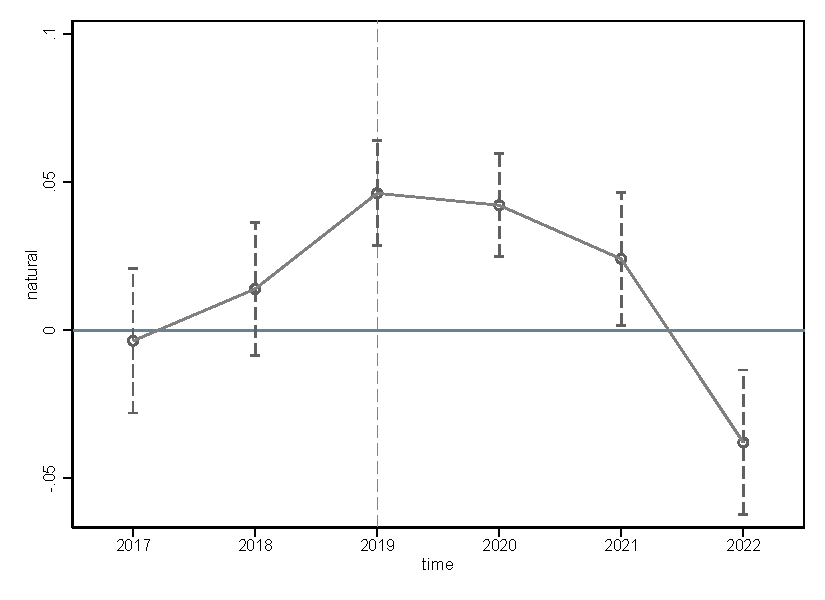
\includegraphics[width=0.5\textwidth]{../figures/did_1.pdf}\label{fig:did_income}}
    \subfloat[Effect to number of house tours]{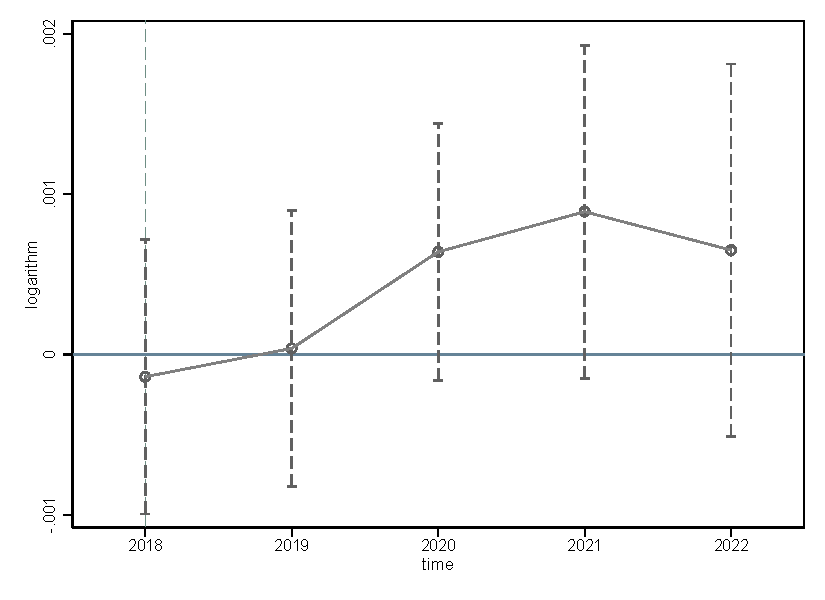
\includegraphics[width=0.5\textwidth]{../figures/did_2.pdf}\label{fig:did_lead_times}}
    \hfill % Adds horizontal space between figures
    \subfloat[Effect to transaction period]{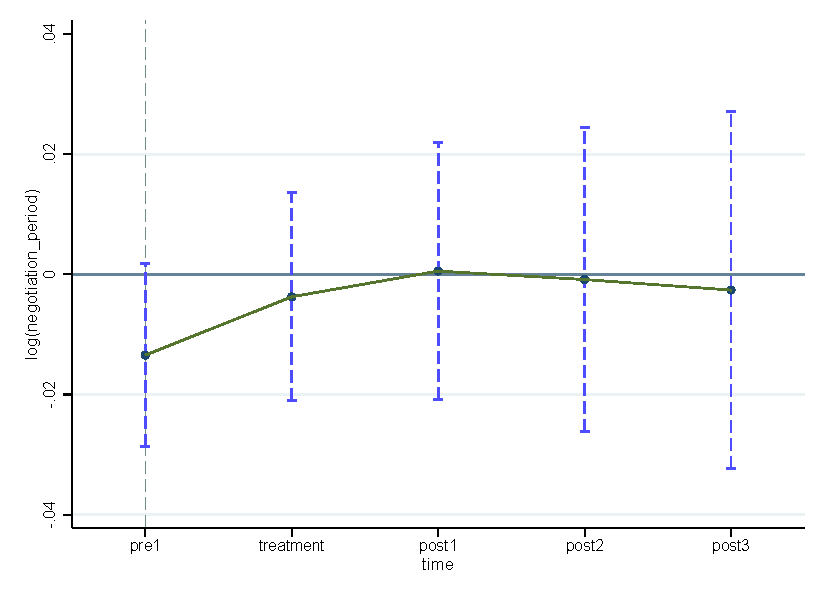
\includegraphics[width=0.5\textwidth]{../figures/did_3.pdf}\label{fig:negotiation_period}}
    \subfloat[Effect to price concession]{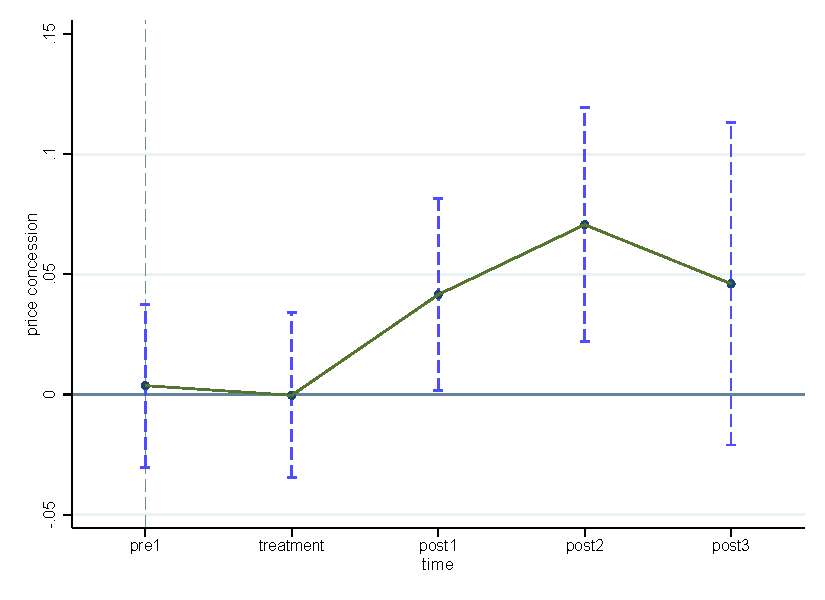
\includegraphics[width=0.5\textwidth]{../figures/did_4.pdf}\label{fig:did_price_concession}}
    \caption{Estimation of Platform Consolidation Effect}
    \label{fig:dynamic_effect}
\end{figure}

The empirical findings indicate that in the first year of the consolidation strategy, Lianjia's transaction revenue did not show a statistically significant difference. However, after the first year, the transaction revenue demonstrated a significant positive increase, ranging from 3\% to 6\%. Additionally, the platform consolidation had a significantly positive impact on the number of house tours, with effects following the same trend as the transaction revenue. Furthermore, when comparing the effect of platform consolidation with the entry effect of offline stores, the result indicates that the effect is substantially more pronounced and more continuous. These results underscore the superior efficacy of platform consolidation in enhancing market performance and provide compelling evidence for the strategic advantage of platformization over traditional offline expansion.

However, in terms of the transaction period, the platformization strategy does not exhibit a significant effect, indicating that platformization does not assist brokerages in facilitating better matching and negotiation between sellers and buyers. Moreover, in terms of the platform's consolidation effect on price concessions, we find that the effect is significant after the first period, with a 4.2\% increase in the first year after the treatment and a 7.1\% increase in the second year. However, the effect becomes insignificant after the third year. Overall, the results show that comparing with the offline store's entry effect, the platform's consolidation strategy can have more pronounced influence not only on effectiveness on trasaction but also on the overall revenue.

revise the paragraph to make it more economics and academic
( this is today's work )

While the platformization strategy is less effective in influencing individuals' decision-making processes compared to offline store entry, it proves more effective in increasing revenue and the number of house tours. This discrepancy highlights that the platformization strategy excels in attracting customers and generating revenue, but falls short in aiding the matching and negotiation process. These findings align with the intuition that platformization is more likely to draw customers and boost revenue, yet it is less effective in assisting buyers and sellers in reaching agreements.

To further investigate the impact of market concentration on the effectiveness of the platformization strategy, we classified the samples into high and low Herfindahl-Hirschman Index (HHI) groups and estimated the model separately for each group. The high HHI group, representing markets with higher concentration, revealed that the platformization strategy does not confer significant benefits for Lianjia's operations. Conversely, in the low HHI group, indicative of less competitive markets, the platformization strategy significantly increases revenue. This suggests that the platformization strategy is more effective in less competitive markets, enhancing Lianjia's competitiveness. In terms of the number of house tours, the effect of platformization is consistent across both high and low HHI groups. This consistency aligns with the intuition that consumer preferences for different types of brokerages are similar, and individuals are equally likely to search for houses online regardless of the brokerage's market share. Moreover, our analysis in columns 5 to 8 shows that the platformization strategy does not have a significant effect on the transaction period or price concessions. This finding suggests that the platformization strategy does not facilitate better matching between buyers and sellers or improve the negotiation process. This aligns with the intuition that while the platformization strategy can attract more customers and generate revenue, it does not inherently improve the efficiency of matching buyers and sellers or negotiating terms because most of the transactions are still offline based.

\begin{table}
  \begin{center}
    \begin{scriptsize}
      \caption{Robustness Check of Online Consolidation Effect}
      \label{tab:heter_platform_did}
      {
\def\sym#1{\ifmmode^{#1}\else\(^{#1}\)\fi}
\begin{tabular}{l*{6}{c}}
\toprule
            &\multicolumn{1}{c}{(1)}&\multicolumn{1}{c}{(2)}&\multicolumn{1}{c}{(3)}&\multicolumn{1}{c}{(4)}&\multicolumn{1}{c}{(5)}&\multicolumn{1}{c}{(6)}\\
            &\multicolumn{1}{c}{log(income)}&\multicolumn{1}{c}{log(income)}&\multicolumn{1}{c}{log(income)}&\multicolumn{1}{c}{log(lead times)}&\multicolumn{1}{c}{log(lead times)}&\multicolumn{1}{c}{log(lead times)}\\
\midrule
pre1\_treatment&      -0.019         &      -0.012         &       0.021         &       0.017         &       0.015         &      -0.044\sym{**} \\
            &     (0.021)         &     (0.016)         &     (0.030)         &     (0.015)         &     (0.013)         &     (0.019)         \\
\addlinespace
treatment   &      -0.033\sym{*}  &      -0.002         &       0.020         &       0.006         &      -0.002         &      -0.017         \\
            &     (0.018)         &     (0.017)         &     (0.033)         &     (0.016)         &     (0.013)         &     (0.022)         \\
\addlinespace
post1\_treatment&       0.038\sym{*}  &       0.072\sym{***}&       0.051         &       0.046\sym{**} &       0.035\sym{**} &      -0.006         \\
            &     (0.022)         &     (0.019)         &     (0.036)         &     (0.018)         &     (0.014)         &     (0.024)         \\
\addlinespace
post2\_treatment&       0.059\sym{***}&       0.080\sym{***}&       0.031         &       0.040\sym{*}  &       0.028\sym{*}  &      -0.007         \\
            &     (0.023)         &     (0.021)         &     (0.041)         &     (0.021)         &     (0.016)         &     (0.024)         \\
\addlinespace
post3\_treatment&      -0.002         &       0.069\sym{***}&       0.046         &       0.027         &      -0.006         &       0.025         \\
            &     (0.026)         &     (0.025)         &     (0.070)         &     (0.023)         &     (0.019)         &     (0.028)         \\
\addlinespace
broker\_410  &      -0.001         &      -0.001         &       0.008\sym{*}  &      -0.001         &       0.002         &      -0.005         \\
            &     (0.002)         &     (0.002)         &     (0.005)         &     (0.001)         &     (0.002)         &     (0.003)         \\
\addlinespace
ln\_end\_price&       0.895\sym{***}&       0.849\sym{***}&       1.019\sym{***}&       0.181\sym{***}&       0.204\sym{***}&      -0.311\sym{***}\\
            &     (0.039)         &     (0.045)         &     (0.073)         &     (0.034)         &     (0.038)         &     (0.033)         \\
\addlinespace
ln\_watch\_people&       0.042\sym{***}&       0.046\sym{***}&       0.028\sym{***}&       0.340\sym{***}&       0.342\sym{***}&       0.366\sym{***}\\
            &     (0.006)         &     (0.006)         &     (0.009)         &     (0.008)         &     (0.007)         &     (0.004)         \\
\addlinespace
ln\_watch\_time&       0.019\sym{***}&       0.024\sym{***}&       0.034\sym{***}&       0.026\sym{***}&       0.028\sym{***}&       0.035\sym{***}\\
            &     (0.003)         &     (0.003)         &     (0.004)         &     (0.003)         &     (0.003)         &     (0.002)         \\
\addlinespace
ln\_nego\_changes&       0.023\sym{***}&       0.010         &       0.017         &       0.115\sym{***}&       0.128\sym{***}&       0.668\sym{***}\\
            &     (0.009)         &     (0.010)         &     (0.016)         &     (0.012)         &     (0.010)         &     (0.009)         \\
\addlinespace
ln\_negotiation\_period&       0.064\sym{***}&       0.075\sym{***}&       0.089\sym{***}&       0.086\sym{***}&       0.123\sym{***}&                     \\
            &     (0.005)         &     (0.005)         &     (0.010)         &     (0.006)         &     (0.006)         &                     \\
\midrule
\(N\)       &       41849         &       53806         &       24273         &       41849         &       53806         &      468936         \\
R-squared   &       0.896         &       0.902         &       0.919         &       0.935         &       0.927         &       0.528         \\
\bottomrule
\multicolumn{7}{l}{\footnotesize Standard errors in parentheses}\\
\multicolumn{7}{l}{\footnotesize \sym{*} \(p<0.1\), \sym{**} \(p<0.05\), \sym{***} \(p<0.01\)}\\
\end{tabular}
}

    
    Note: we omit all the control variables in the regression model, and detailed descriptions can be seen from Table \ref{tab:statistical_district} and Table \ref{tab:statistical_individual}.
    \end{scriptsize}
  \end{center}
\end{table}

\begin{table}
  \begin{center}
    \begin{scriptsize}
      \caption{Robustness Check of Online Consolidation Effect (Continued)}
      \label{tab:heter_platform_did}
      {
\def\sym#1{\ifmmode^{#1}\else\(^{#1}\)\fi}
\begin{adjustbox}{max width=\textwidth}
\begin{tabular}{l*{6}{c}}
\toprule
            &\multicolumn{1}{c}{(1)}&\multicolumn{1}{c}{(2)}&\multicolumn{1}{c}{(3)}&\multicolumn{1}{c}{(4)}&\multicolumn{1}{c}{(5)}&\multicolumn{1}{c}{(6)}\\
            &\multicolumn{1}{c}{log(negotiation period)}&\multicolumn{1}{c}{log(negotiation period)}&\multicolumn{1}{c}{log(negotiation period)}&\multicolumn{1}{c}{price concession}&\multicolumn{1}{c}{price concession}&\multicolumn{1}{c}{price concession}\\
\midrule
pre1\_treatment&       0.001         &      -0.002         &      -0.044\sym{*}  &       0.012         &      -0.011         &      -0.017         \\
            &     (0.017)         &     (0.016)         &     (0.025)         &     (0.041)         &     (0.034)         &     (0.049)         \\
\addlinespace
treatment   &       0.001         &      -0.004         &       0.014         &       0.017         &      -0.017         &      -0.019         \\
            &     (0.021)         &     (0.016)         &     (0.030)         &     (0.041)         &     (0.036)         &     (0.060)         \\
\addlinespace
post1\_treatment&       0.001         &      -0.015         &       0.005         &       0.084\sym{*}  &       0.026         &       0.020         \\
            &     (0.025)         &     (0.020)         &     (0.031)         &     (0.050)         &     (0.041)         &     (0.066)         \\
\addlinespace
post2\_treatment&      -0.002         &      -0.022         &      -0.013         &       0.160\sym{***}&       0.068         &       0.092         \\
            &     (0.027)         &     (0.023)         &     (0.029)         &     (0.056)         &     (0.048)         &     (0.077)         \\
\addlinespace
post3\_treatment&      -0.004         &      -0.011         &       0.026         &       0.034         &       0.118\sym{*}  &      -0.086         \\
            &     (0.031)         &     (0.026)         &     (0.040)         &     (0.067)         &     (0.067)         &     (0.130)         \\
\addlinespace
other brokerage num  &      -0.001         &      -0.000         &      -0.003         &      -0.008\sym{***}&      -0.001         &       0.002         \\
            &     (0.001)         &     (0.002)         &     (0.004)         &     (0.003)         &     (0.004)         &     (0.010)         \\
\addlinespace
ln(Price)&      -0.111\sym{***}&      -0.243\sym{***}&      -0.334\sym{***}&       1.246\sym{***}&       1.365\sym{***}&       1.636\sym{***}\\
            &     (0.032)         &     (0.025)         &     (0.035)         &     (0.080)         &     (0.083)         &     (0.120)         \\
\addlinespace
log(watch people)&       0.362\sym{***}&       0.368\sym{***}&       0.367\sym{***}&       0.090\sym{***}&       0.060\sym{***}&       0.037\sym{***}\\
            &     (0.005)         &     (0.004)         &     (0.005)         &     (0.006)         &     (0.006)         &     (0.007)         \\
\addlinespace
log(watch time)&       0.041\sym{***}&       0.038\sym{***}&       0.035\sym{***}&      -0.052\sym{***}&      -0.056\sym{***}&      -0.058\sym{***}\\
            &     (0.003)         &     (0.002)         &     (0.003)         &     (0.005)         &     (0.004)         &     (0.005)         \\
\addlinespace
log(nego changes)&       0.653\sym{***}&       0.663\sym{***}&       0.665\sym{***}&       0.177\sym{***}&       0.159\sym{***}&       0.173\sym{***}\\
            &     (0.008)         &     (0.007)         &     (0.010)         &     (0.009)         &     (0.008)         &     (0.011)         \\
\midrule
\(N\)       &      333284         &      587056         &      345003         &      328031         &      576728         &      338698         \\
R-squared   &       0.548         &       0.538         &       0.529         &       0.255         &       0.247         &       0.270         \\
\bottomrule
\multicolumn{7}{l}{\footnotesize Standard errors in parentheses}\\
\multicolumn{7}{l}{\footnotesize \sym{*} \(p<0.1\), \sym{**} \(p<0.05\), \sym{***} \(p<0.01\)}\\
\end{tabular}
\end{adjustbox}
}

    
    Note: we omit all the control variables in the regression model, and detailed descriptions can be seen from Table \ref{tab:statistical_district} and Table \ref{tab:statistical_individual}.
    \end{scriptsize}
  \end{center}
\end{table}


In the online Appendix \ref{tab:platform_consolidation_hetero_mature}, we present the heterogeneous effects of Lianjia's operations in both mature and immature markets. Figure \ref{fig:treatment_consolidation} illustrates the distribution of income across the treatment and control groups. Prior to the intervention, the two groups exhibit parallel trends, indicating no significant differences. The treatment effect becomes significant only after the first period, aligning with our empirical findings.


















The result is consistent with the opinion that most platform like uber and lyft that does not have enough network strength and \citep{10.1257/jep.28.2.3}

\citep{WOS:000454186600016}

\section{Extension: Collaborative Spillover Effect} \label{sec:network_effect}

The last section is to estimate the Lianjia's collaborative spillover effect. Lianjia decided to change from brokerage's direction operation to a combination of platform. By attracting other brokerage's into the network will initially make the brokreage's profit down because attracting other people in the platform meaning the market share would be decreased due to the intense competition. However, after the setup of the platform, the market will be more productive and more competitive to occupying a larger share of the whole network. This mechanism is more likely to get better control over the listing and people are more willing to list their house on this platform. Then accordin to the this would be resulted in a winners-take-all market.

In this case, we need to empirically estimate the spillover effect, and if this spillover effect is significant in this setting then people's reaction 

To set up, we first match the brokerages' with the 


We decided to use the so called quantile estimator described in model  proposed by \citep{machado_quantiles_2019}.

\begin{equation}
  \begin{aligned}
    Q_y(\xi \mid X) & = \beta_0 + \beta_1(\xi) \text{pre\_treatment}_{it} + \beta_2(\xi) \text{treatment} + \sum_{i=3}^5 \beta_i(\xi) \text{post\_treatment}_{it} \\
    & + \beta(\xi) \bf{X}_{it} + \mu_i + \tau_t + \varepsilon_{it}
  \end{aligned}
\end{equation}

\ref{tab:quantile_estimate_network} shows the quantile estimation of the . We can see that the 





\begin{figure}
  \centering
  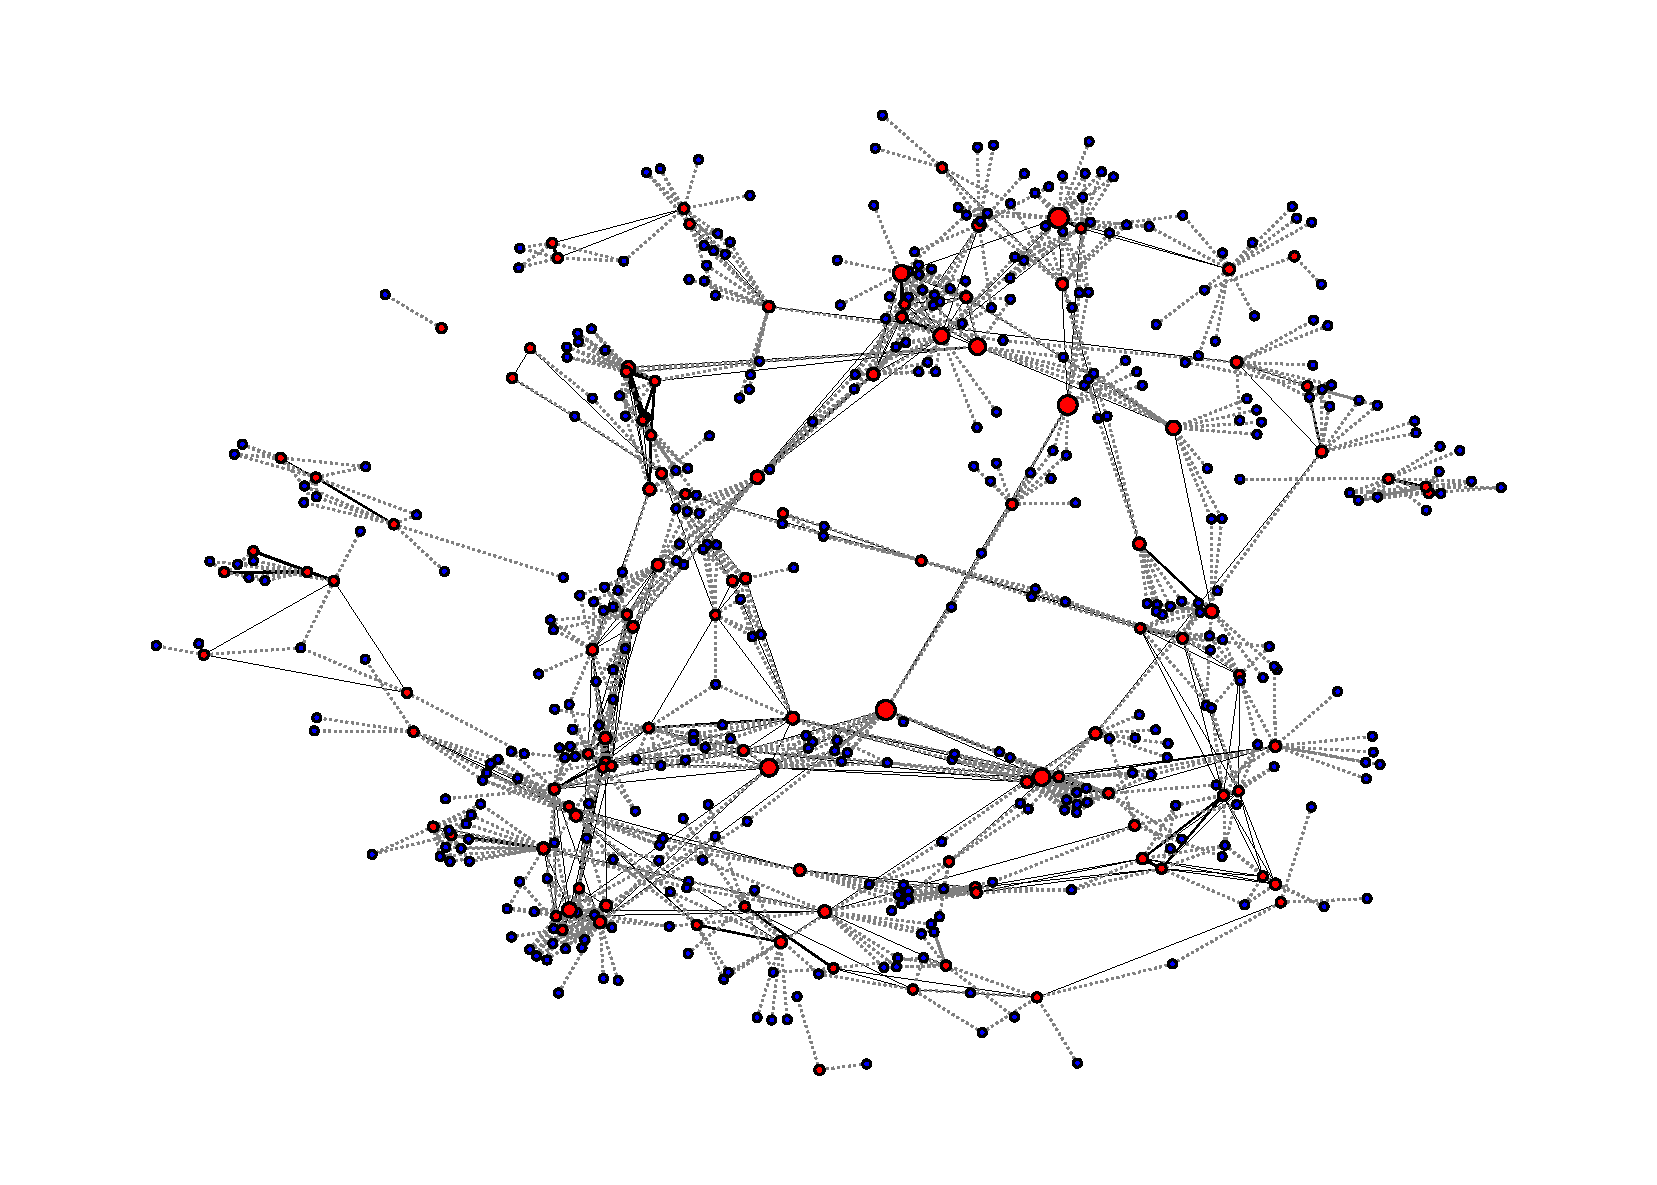
\includegraphics[width=0.7\textwidth]{../figures/network_formation_effect.pdf}
  \caption{The structure of network formation effect}
  \label{fig:network_formation_effect_graph}

  Note: The red nodes represent the distribution of Lianjia's offline stores, while the blue nodes indicate the distribution of neighborhoods within the market. Dotted edges illustrate the connections between neighborhoods and stores, whereas solid lines depict the interactions between offline stores. The size of the red nodes corresponds to the local clustering effect, with larger nodes indicating a more significant local clustering phenomenon.
\end{figure}

\begin{table}
  \begin{center}
    \begin{scriptsize}
      \caption{Estimated Network Spillover Effect}
      \label{tab:estiamted_spillover_effect}
      \begin{tabular}{lllllllll}
\hline
 city      & index                    & 2016   & 2017   & 2018   & 2019   & 2020   & 2021    & 2022   \\
\hline
 Beijing   & average local clustering & 0.15   & 0.18   & 0.19   & 0.19   & 0.20   &         &        \\
 Beijing   & global clustering        & 0.30   & 0.36*  & 0.38*  & 0.38*  & 0.41*  &         &        \\
 Chengdu   & average local clustering & 0.20   & 0.21   & 0.20   & 0.22   & 0.23   &         &        \\
 Chengdu   & global clustering        & 0.29   & 0.29   & 0.33*  & 0.35*  & 0.38*  &         &        \\
 Chongqing & average local clustering & 0.09   & 0.13   & 0.14   & 0.16   & 0.21   & 0.23    & 0.24   \\
 Chongqing & global clustering        & 0.20   & 0.24   & 0.28   & 0.31*  & 0.44*  & 0.52**  & 0.56** \\
 Guangzhou & average local clustering & 0.06   & 0.16   & 0.17   & 0.16   & 0.24   & 0.27    & 0.28   \\
 Guangzhou & global clustering        & 0.12   & 0.33*  & 0.40*  & 0.31*  & 0.43*  & 0.53**  & 0.57** \\
 Hangzhou  & average local clustering & 0.14   & 0.16   & 0.16   & 0.18   & 0.25   & 0.25    & 0.24   \\
 Hangzhou  & global clustering        & 0.24   & 0.32*  & 0.35*  & 0.34*  & 0.46*  & 0.48*   & 0.51** \\
 Nanjing   & average local clustering & 0.16   & 0.23   & 0.23   & 0.23   & 0.25   & 0.25    & 0.25   \\
 Nanjing   & global clustering        & 0.29   & 0.42*  & 0.44*  & 0.43*  & 0.46*  & 0.48*   & 0.50*  \\
 Shanghai  & average local clustering & 0.21   & 0.21   & 0.20   & 0.21   & 0.19   & 0.18    & 0.18   \\
 Shanghai  & global clustering        & 0.35*  & 0.43*  & 0.43*  & 0.40*  & 0.33*  & 0.34*   & 0.39*  \\
 Shenzhen  & average local clustering & 0.14   & 0.22   & 0.21   & 0.18   & 0.25   &         &        \\
 Shenzhen  & global clustering        & 0.27   & 0.40*  & 0.40*  & 0.37*  & 0.49*  &         &        \\
 Tianjin   & average local clustering & 0.13   & 0.16   & 0.16   & 0.19   & 0.24   & 0.24    & 0.24   \\
 Tianjin   & global clustering        & 0.20   & 0.28   & 0.27   & 0.32*  & 0.43*  & 0.46*   & 0.47*  \\
 Wuhan     & average local clustering & 0.09   & 0.15   & 0.17   & 0.19   & 0.25   &         &        \\
 Wuhan     & global clustering        & 0.26   & 0.38*  & 0.44*  & 0.41*  & 0.55** &         &        \\
\hline
\end{tabular}

      Note: The indices used are the Average and Global Clustering Coefficients. $*$ denotes a low network effect, which ranges from 0.3 to 0.5. $**$ indicates a moderate network effect, ranging from 0.5 to 0.75. $***$ signifies a large network effect, ranging from 0.75 to 1.
    \end{scriptsize}
  \end{center}
\end{table}


\begin{table}
  \begin{center}
    \begin{scriptsize}
      \caption{Quantile Estimation of the Network Spillover Effect}
      \label{tab:quantile_estimate_network}
      {
\def\sym#1{\ifmmode^{#1}\else\(^{#1}\)\fi}
\begin{adjustbox}{max width=\textwidth}
\begin{tabular}{l*{19}{c}}
\toprule
            &\multicolumn{1}{c}{(1)}&\multicolumn{1}{c}{(2)}&\multicolumn{1}{c}{(3)}&\multicolumn{1}{c}{(4)}&\multicolumn{1}{c}{(5)}&\multicolumn{1}{c}{(6)}&\multicolumn{1}{c}{(7)}&\multicolumn{1}{c}{(8)}&\multicolumn{1}{c}{(9)}&\multicolumn{1}{c}{(10)}&\multicolumn{1}{c}{(11)}&\multicolumn{1}{c}{(12)}&\multicolumn{1}{c}{(13)}&\multicolumn{1}{c}{(14)}&\multicolumn{1}{c}{(15)}&\multicolumn{1}{c}{(16)}&\multicolumn{1}{c}{(17)}&\multicolumn{1}{c}{(18)}&\multicolumn{1}{c}{(19)}\\
            &\multicolumn{1}{c}{} &\multicolumn{1}{c}{quantile\_10}&\multicolumn{1}{c}{quantile\_15}&\multicolumn{1}{c}{quantile\_20}&\multicolumn{1}{c}{quantile\_25}&\multicolumn{1}{c}{quantile\_30}&\multicolumn{1}{c}{quantile\_35}&\multicolumn{1}{c}{quantile\_40}&\multicolumn{1}{c}{quantile\_45}&\multicolumn{1}{c}{quantile\_50}&\multicolumn{1}{c}{quantile\_55}&\multicolumn{1}{c}{quantile\_60}&\multicolumn{1}{c}{quantile\_65}&\multicolumn{1}{c}{quantile\_70}&\multicolumn{1}{c}{quantile\_75}&\multicolumn{1}{c}{quantile\_80}&\multicolumn{1}{c}{quantile\_85}&\multicolumn{1}{c}{quantile\_90}&\multicolumn{1}{c}{quantile\_95}\\
\midrule
pre1\_treatment&       0.034         &       0.017         &       0.005         &      -0.003         &      -0.009         &      -0.017         &      -0.026         &      -0.037         &      -0.049         &      -0.062         &      -0.076         &      -0.089         &      -0.101         &      -0.111         &      -0.119         &      -0.127         &      -0.139         &      -0.153         &      -0.173         \\
            &     (0.584)         &     (0.518)         &     (0.473)         &     (0.441)         &     (0.416)         &     (0.388)         &     (0.352)         &     (0.312)         &     (0.267)         &     (0.216)         &     (0.166)         &     (0.124)         &     (0.092)         &     (0.078)         &     (0.080)         &     (0.095)         &     (0.128)         &     (0.173)         &     (0.247)         \\
\addlinespace
treatment   &       0.878         &       0.860\sym{*}  &       0.848\sym{*}  &       0.840\sym{**} &       0.833\sym{**} &       0.826\sym{**} &       0.816\sym{**} &       0.805\sym{***}&       0.793\sym{***}&       0.779\sym{***}&       0.764\sym{***}&       0.751\sym{***}&       0.739\sym{***}&       0.728\sym{***}&       0.720\sym{***}&       0.711\sym{***}&       0.699\sym{***}&       0.685\sym{***}&       0.664\sym{***}\\
            &     (0.553)         &     (0.491)         &     (0.448)         &     (0.417)         &     (0.394)         &     (0.368)         &     (0.333)         &     (0.295)         &     (0.252)         &     (0.205)         &     (0.157)         &     (0.117)         &     (0.087)         &     (0.073)         &     (0.076)         &     (0.090)         &     (0.121)         &     (0.164)         &     (0.233)         \\
\addlinespace
post1\_treatment&       1.433\sym{**} &       1.398\sym{**} &       1.373\sym{***}&       1.356\sym{***}&       1.343\sym{***}&       1.328\sym{***}&       1.308\sym{***}&       1.286\sym{***}&       1.261\sym{***}&       1.233\sym{***}&       1.204\sym{***}&       1.177\sym{***}&       1.152\sym{***}&       1.129\sym{***}&       1.114\sym{***}&       1.096\sym{***}&       1.071\sym{***}&       1.044\sym{***}&       1.001\sym{***}\\
            &     (0.650)         &     (0.577)         &     (0.527)         &     (0.491)         &     (0.463)         &     (0.432)         &     (0.392)         &     (0.347)         &     (0.297)         &     (0.240)         &     (0.185)         &     (0.138)         &     (0.102)         &     (0.086)         &     (0.090)         &     (0.106)         &     (0.142)         &     (0.192)         &     (0.274)         \\
\addlinespace
post2\_treatment&       1.626\sym{**} &       1.625\sym{**} &       1.624\sym{**} &       1.623\sym{***}&       1.622\sym{***}&       1.622\sym{***}&       1.621\sym{***}&       1.620\sym{***}&       1.619\sym{***}&       1.618\sym{***}&       1.617\sym{***}&       1.616\sym{***}&       1.615\sym{***}&       1.614\sym{***}&       1.613\sym{***}&       1.613\sym{***}&       1.612\sym{***}&       1.610\sym{***}&       1.609\sym{***}\\
            &     (0.802)         &     (0.712)         &     (0.650)         &     (0.605)         &     (0.572)         &     (0.533)         &     (0.483)         &     (0.428)         &     (0.366)         &     (0.297)         &     (0.228)         &     (0.170)         &     (0.126)         &     (0.106)         &     (0.110)         &     (0.130)         &     (0.175)         &     (0.237)         &     (0.338)         \\
\addlinespace
post3\_treatment&       1.689         &       1.697         &       1.702         &       1.705\sym{*}  &       1.708\sym{*}  &       1.711\sym{**} &       1.715\sym{**} &       1.720\sym{**} &       1.725\sym{***}&       1.731\sym{***}&       1.737\sym{***}&       1.742\sym{***}&       1.747\sym{***}&       1.752\sym{***}&       1.755\sym{***}&       1.759\sym{***}&       1.764\sym{***}&       1.770\sym{***}&       1.779\sym{***}\\
            &     (1.281)         &     (1.137)         &     (1.039)         &     (0.967)         &     (0.913)         &     (0.852)         &     (0.772)         &     (0.684)         &     (0.585)         &     (0.474)         &     (0.365)         &     (0.271)         &     (0.202)         &     (0.170)         &     (0.176)         &     (0.208)         &     (0.280)         &     (0.379)         &     (0.541)         \\
\midrule
\(N\)       &      142734         &      142734         &      142734         &      142734         &      142734         &      142734         &      142734         &      142734         &      142734         &      142734         &      142734         &      142734         &      142734         &      142734         &      142734         &      142734         &      142734         &      142734         &      142734         \\
\bottomrule
\multicolumn{20}{l}{\footnotesize Standard errors in parentheses}\\
\multicolumn{20}{l}{\footnotesize \sym{*} \(p<0.1\), \sym{**} \(p<0.05\), \sym{***} \(p<0.01\)}\\
\end{tabular}
\end{adjustbox}
}

    
    Note: we omit all the control variables in the regression model, and detailed descriptions can be seen from Table \ref{tab:statistical_district} and Table \ref{tab:statistical_individual}.
    \end{scriptsize}
  \end{center}
\end{table}


















\section{Conclusion and Discussion} \label{sec:conclusion}

In the China's real estate market the 

The Chinese real estate market witnessed a significnat drop at 2022 and the labor market is fierece in recently and therefore, the people are pretty hard to get on jobs.

The study of Lianjia's strategic expansion into China's real estate brokerage industry, particularly through the implementation of the ACN and the proliferation of offline branches, underscores a transformative impact on market dynamics and transaction efficiency. Our empirical research shows that Lianjia's approach, which seamlessly integrates online platforms with an extensive offline presence, significantly enhances revenue generation and influences consumer behavior, particularly through improved price concessions and increased home viewing. The study highlights the critical role of offline store information and community proximity in increasing transaction revenue and achieving market dominance, even in the face of increasing monopolization trends. Despite the adverse effects of the COVID-19 pandemic, which temporarily diluted the benefits of both customer base expansion and information dissemination, the resilience of physical stores emerges prominently. This resilience, coupled with the strategic leverage of online platforms, underscores the importance of a synergistic online-offline model in overcoming market challenges and maintaining competitive advantage. The findings argue for a nuanced understanding of platform-based monopolization in real estate, suggesting that the successful integration of digital and physical domains can significantly enhance service delivery, market penetration, and overall system competitiveness, paving the way for a more adaptive and robust market system in the face of evolving challenges.

%%%%%%%%%%%%%%%%%%%%%%%%%%%%%%%%%%%%%%%%%%%%%%%%%
\clearpage
\begin{singlespace}
%\bibliographystyle{plainnat}
%\bibliographystyle{chicago}
% \bibliographystyle{aer}
% \bibliography{our-cites.bib}

\begin{thebibliography}{}

  \bibitem[Bailey et al.(2018)]{bailey_economic_2018}
  Bailey, M., R. Cao, T. Kuchler, and J. Stroebel. 2018. The Economic Effects of Social Networks: Evidence from the Housing Market. \textit{Journal of Political Economy}, 126(6), 2224-2276.
  
  \bibitem[Rosen(1974)]{Rosen_hedonic}
  Rosen, S. 1974. Hedonic Prices and Implicit Markets: Product Differentiation in Pure Competition. \textit{Journal of Political Economy}, 82(1), 34-55.% Available at \url{http://www.jstor.org/stable/1830899}.
  
  \bibitem[Chen and Wen(2017)]{chen_great_2017}
  Chen, K., and Y. Wen. 2017. The Great Housing Boom of China. \textit{American Economic Journal: Macroeconomics}, 9(2), 73-114.
  
  \bibitem[Farrell and Shapiro(1990)]{farrell_horizontal_1990}
  Farrell, J., and C. Shapiro. 1990. Horizontal Mergers: An Equilibrium Analysis. \textit{American Economic Review}, 80(1), 107-126.
  
  \bibitem[Athey and Imbens(2016)]{athey_recursive_2016}
  Athey, S., and G. Imbens. 2016. Recursive Partitioning for Heterogeneous Causal Effects. \textit{Proceedings of the National Academy of Sciences of the United States of America}, 113(27), 7353-7360.
  
  \bibitem[d'Aspremont et al.(1979)]{daspremont_hotellings_1979}
  d'Aspremont, C., J. J. Gabszewicz, and J.-F. Thisse. 1979. On Hotelling’s "Stability in Competition". \textit{Econometrica}, 47(5), 1145-1150.
  
  \bibitem[Glaeser et al.(2017)]{glaeser_real_2017}
  Glaeser, E., W. Huang, Y. Ma, and A. Shleifer. 2017. A Real Estate Boom with Chinese Characteristics. \textit{Journal of Economic Perspectives}, 31(1), 93-116.
  
  \bibitem[Grossman and Stiglitz(1980)]{grossman_impossibility_1980}
  Grossman, S. J., and J. E. Stiglitz. 1980. On the Impossibility of Informationally Efficient Markets. \textit{American Economic Review}, 70(3), 393-408.
  
  \bibitem[Handbury(2021)]{handbury_are_2021}
  Handbury, J. 2021. Are Poor Cities Cheap for Everyone? Non-Homotheticity and the Cost of Living Across U.S. Cities. \textit{Econometrica}, 89(6), 2679-2715.
  
  \bibitem[Hendel et al.(2009)]{hendel_relative_2009}
  Hendel, I., A. Nevo, and F. Ortalo-Magné. 2009. The Relative Performance of Real Estate Marketing Platforms: MLS versus FSBOMadison.com. \textit{American Economic Review}, 99(5), 1878-1898.
  
  \bibitem[Hotelling(1929)]{hotelling_stability_1929}
  Hotelling, H. 1929. The Stability in Competition. \textit{Economic Journal}, 39, 41-57.
  
  \bibitem[Hsieh and Moretti(2003)]{hsieh_can_2003}
  Hsieh, C.-T., and E. Moretti. 2003. Can Free Entry Be Inefficient? Fixed Commissions and Social Waste in the Real Estate Industry. \textit{Journal of Political Economy}, 111(5), 1076-1122.
  
  \bibitem[Hui and Chan(2014)]{hui_foreign_2014}
  Hui, E. C. M., and K. K. K. Chan. 2014. Foreign Direct Investment in China's Real Estate Market. \textit{Habitat International}, 43, 231-239.
  
  \bibitem[Piazzesi et al.(2020)]{piazzesi_segmented_2020}
  Piazzesi, M., M. Schneider, and J. Stroebel. 2020. Segmented Housing Search. \textit{American Economic Review}, 110(3), 720-759.
  
  \bibitem[Qu et al.(2021)]{qu_identifying_2021}
  Qu, W., Y. Huang, and G. Deng. 2021. Identifying the Critical Factors Behind the Second-Hand Housing Price Concession: Empirical Evidence from China. \textit{Habitat International}, 117, 102442.
  
  \bibitem[Salz(2022)]{salz_intermediation_2022}
  Salz, T. 2022. Intermediation and Competition in Search Markets: An Empirical Case Study. \textit{Journal of Political Economy}, 130(2), 310-345.
  
  \bibitem[Williams(1998)]{williams_agency_1998}
  Williams, J. T. 1998. Agency and Brokerage of Real Assets in Competitive Equilibrium. \textit{Review of Financial Studies}, 11(2), 239-280.
  
  \bibitem[Wong et al.(2012)]{wong_liquidity_2012}
  Wong, S. K., C. Y. Yiu, and K. W. Chau. 2012. Liquidity and Information Asymmetry in the Real Estate Market. \textit{The Journal of Real Estate Finance and Economics}, 45(1), 49-62.
  
  \bibitem[Zhao(2015)]{zhao_rational_2015}
  Zhao, B. 2015. Rational Housing Bubble. \textit{Economic Theory}, 60(1), 141-201.
  
  \bibitem[Elvidge et al.(2021)]{elvidge_annual_2021}
  Elvidge, C. D., M. Zhizhin, T. Ghosh, F.-C. Hsu, and J. Taneja. 2021. Annual Time Series of Global VIIRS Nighttime Lights Derived from Monthly Averages: 2012 to 2019. \textit{Remote Sensing}, 13(5), 922.
  
  \bibitem[Zhang et al.(2021)]{zhang_online_2021}
  Zhang, X., Z. Lin, Y. Zhang, Y. Zheng, and J. Zhang. 2021. Online Property Brokerage Platform and Prices of Second-Hand Houses: Evidence from Lianjia's Entry. \textit{Electronic Commerce Research and Applications}, 50, 101104.
  
  \bibitem[Wei and Zhang(2011)]{wei_competitive_2011}
  Wei, S.-J., and X. Zhang. 2011. The Competitive Saving Motive: Evidence from Rising Sex Ratios and Savings Rates in China. \textit{Journal of Political Economy}, 119(3), 511-564.
  
  \bibitem[Zhao et al.(2017)]{zhao_forecasting_2017}
  Zhao, N., Y. Liu, G. Cao, E. L. Samson, and J. Zhang. 2017. Forecasting China’s GDP at the Pixel Level Using Nighttime Lights Time Series and Population Images. \textit{GIScience \& Remote Sensing}, 54(3), 407-425.
  
  \bibitem[Akerlof(1970)]{Akerlof_1970}
  Akerlof, G. A. 1970. The Market for "Lemons": Quality Uncertainty and the Market Mechanism. \textit{The Quarterly Journal of Economics}, 84(3), 488-500.
  
  \bibitem[Yang et al.(2021)]{YANG2021102359}
  Yang, L., K. W. Chau, and Y. Chen. 2021. Impacts of Information Asymmetry and Policy Shock on Rental and Vacancy Dynamics in Retail Property Markets. \textit{Habitat International}, 111, 102359.
  
  \bibitem[Barwick and Pathak(2015)]{https://doi.org/10.1111/1756-2171.12082}
  Barwick, P. J., and P. A. Pathak. 2015. The Costs of Free Entry: An Empirical Study of Real Estate Agents in Greater Boston. \textit{The RAND Journal of Economics}, 46(1), 103-145.
  
  \bibitem[Barwick et al.(2017)]{10.1257/app.20160214}
  Barwick, P. J., P. A. Pathak, and M. Wong. 2017. Conflicts of Interest and Steering in Residential Brokerage. \textit{American Economic Journal: Applied Economics}, 9(3), 191-222.
  
  \bibitem[Levitt and Syverson(2008)]{d082a2db-5cce-33f2-87c4-9cb020cc6666}
  Levitt, S. D., and C. Syverson. 2008. Market Distortions When Agents Are Better Informed: The Value of Information in Real Estate Transactions. \textit{The Review of Economics and Statistics}, 90(4), 599-611.
  
  \bibitem[Pope et al.(2015)]{POPE201589}
  Pope, D. G., J. C. Pope, and J. R. Sydnor. 2015. Focal Points and Bargaining in Housing Markets. \textit{Games and Economic Behavior}, 93, 89-107.
  
  \bibitem[Han and Strange(2015)]{HAN2015813}
  Han, L., and W. C. Strange. 2015. The Microstructure of Housing Markets: Search, Bargaining, and Brokerage. In \textit{Handbook of Regional and Urban Economics}, Vol. 5, pp. 813-886. Elsevier.
  
  \bibitem[Genesove and Han(2012)]{GENESOVE201231}
  Genesove, D., and L. Han. 2012. Search and Matching in the Housing Market. \textit{Journal of Urban Economics}, 72(1), 31-45.
  
  \bibitem[Han and Hong(2011)]{550a6ccf-cde2-3dd1-979f-1a8db2b8ceb9}
  Han, L., and S.-H. Hong. 2011. Testing Cost Inefficiency Under Free Entry in the Real Estate Brokerage Industry. \textit{Journal of Business \& Economic Statistics}, 29(4), 564-578.
  
  \bibitem[Van Nieuwerburgh and Veldkamp(2010)]{NIEUWERBURGH_information}
  Van Nieuwerburgh, S., and L. Veldkamp. 2010. Information Acquisition and Under-Diversification. \textit{The Review of Economic Studies}, 77(2), 779-805.
  
  \bibitem[Zhang et al.(2021)]{ZHANG2021101104}
  Zhang, X., Z. Lin, Y. Zhang, Y. Zheng, and J. Zhang. 2021. Online Property Brokerage Platform and Prices of Second-Hand Houses: Evidence from Lianjia’s Entry. \textit{Electronic Commerce Research and Applications}, 50, 101104.
  
  \bibitem[Agarwal et al.(2019)]{AGARWAL2019715}
  Agarwal, S., J. He, T. F. Sing, and C. Song. 2019. Do Real Estate Agents Have Information Advantages in Housing Markets? \textit{Journal of Financial Economics}, 134(3), 715-735.
  
  \bibitem[Piazzesi et al.(2020)]{10.1257/aer.20141772}
  Piazzesi, M., M. Schneider, and J. Stroebel. 2020. Segmented Housing Search. \textit{American Economic Review}, 110(3), 720-759.
  
  \bibitem[Hong(2022)]{https://doi.org/10.1002/jae.2891}
  Hong, S.-H. 2022. Real Estate Agents' Influence on Housing Search. \textit{Journal of Applied Econometrics}, 37(3), 563-582.
  
  \bibitem[Van Donkelaar et al.(2021)]{doi:10.1021/acs.est.1c05309}
  Van Donkelaar, A., M. S. Hammer, L. Bindle, M. Brauer, J. R. Brook, M. J. Garay, N. C. Hsu, O. V. Kalashnikova, R. A. Kahn, C. Lee, R. C. Levy, A. Lyapustin, A. M. Sayer, and R. V. Martin. 2021. Monthly Global Estimates of Fine Particulate Matter and Their Uncertainty. \textit{Environmental Science \& Technology}, 55(22), 15287-15300.
  
  \bibitem[Zumpano et al.(2003)]{ZUMPANO2003134}
  Zumpano, L. V., K. H. Johnson, and R. I. Anderson. 2003. Internet Use and Real Estate Brokerage Market Intermediation. \textit{Journal of Housing Economics}, 12(2), 134-150.
  
  \bibitem[McCrary(2008)]{MCCRARY2008698}
  McCrary, J. 2008. Manipulation of the Running Variable in the Regression Discontinuity Design: A Density Test. \textit{Journal of Econometrics}, 142(2), 698-714.
  
  \bibitem[Sirmans et al.(1991)]{SIRMANS1991207}
  Sirmans, C. F., G. K. Turnbull, and J. D. Benjamin. 1991. The Markets for Housing and Real Estate Broker Services. \textit{Journal of Housing Economics}, 1(3), 207-217.
  
  \bibitem[Armstrong(2006)]{Armstrong2006}
  Armstrong, M. 2006. Competition in Two-Sided Markets. \textit{The RAND Journal of Economics}, 37(3), 668-691.
  
  \bibitem[Beck et al.(2022)]{doi:10.1080/10527001.2021.2016340}
  Beck, J., F. Scott, and A. Yelowitz. 2022. The Impact of Real Estate Agent Specialization and Activity Level on Market Outcomes. \textit{Journal of Housing Research}, 31(2), 163-180.
  
  \bibitem[Jud et al.(1996)]{doi:10.1080/10835547.1996.12090852}
  Jud, D., T. Seaks, and D. Winkler. 1996. Time on the Market: The Impact of Residential Brokerage. \textit{Journal of Real Estate Research}, 12(2), 447-458.
  
  \bibitem[Rochet and Tirole(2003)]{10.1162/154247603322493212}
  Rochet, J.-C., and J. Tirole. 2003. Platform Competition in Two-Sided Markets. \textit{Journal of the European Economic Association}, 1(4), 990-1029.
  
  \bibitem[Li and Qi(2022)]{10.1093/cje/beac054}
  Li, Z., and H. Qi. 2022. Platform Power: Monopolisation and Financialisation in the Era of Big Tech. \textit{Cambridge Journal of Economics}, 46(6), 1289-1314.
  
  \bibitem[Langley and Leyshon(2017)]{Langley_Leyshon_2017}
  Langley, P., and A. Leyshon. 2017. Platform Capitalism: The Intermediation and Capitalisation of Digital Economic Circulation. \textit{Finance and Society}, 3(1), 11-31.
  
  \bibitem[Allen et al.(2023)]{RePEc:kap:jrefec:v:67:y:2023:i:3:d:10.1007_s11146-021-09858-w}
  Allen, M. T., J. D. Benefield, and R. C. Rutherford. 2023. Co-Listing Strategies: Better Transaction Outcomes? \textit{The Journal of Real Estate Finance and Economics}, 67(3), 517-544.
  
  \bibitem[Varian(2014)]{10.1257/jep.28.2.3}
  Varian, H. R. 2014. Big Data: New Tricks for Econometrics. \textit{Journal of Economic Perspectives}, 28(2), 3-28.
  
  \bibitem[Zhu and Iansiti(2019)]{WOS:000454186600016}
  Zhu, F., and M. Iansiti. 2019. Why Some Platforms Thrive and Others Don't. \textit{Harvard Business Review}, 97(1), 118-125.
  
  \bibitem[Athey and Imbens(2006)]{https://doi.org/10.1111/j.1468-0262.2006.00668.x}
  Athey, S., and G. W. Imbens. 2006. Identification and Inference in Nonlinear Difference-in-Differences Models. \textit{Econometrica}, 74(2), 431-497.% Available at \url{https://onlinelibrary.wiley.com/doi/abs/10.1111/j.1468-0262.2006.00668.x}.

  \bibitem[Machado and Santos Silva(2019)]{machado_quantiles_2019}
Machado, J. A. F., and J. M. C. Santos Silva. 2019. Quantiles via Moments. \textit{Journal of Econometrics}, 213(1), 145-173.

  \end{thebibliography}
\end{singlespace}
%%%%%%%%%%%%%%%%%%%%%%%%%%%%%%%%%%%%%%%%%%%%%%%%%


%%%%%%%%%%%%%%%%%%%%%%%%%%%%%%%%%%%%%%%%%%%%%%%%%
%%%%% These commands start the appendix and change the Table & Figure numbering
\newpage
\appendix
\setcounter{table}{0}
\renewcommand{\tablename}{Appendix Table}
\renewcommand{\figurename}{Appendix Figure}
\renewcommand{\thetable}{A\arabic{table}}
\setcounter{figure}{0}
\renewcommand{\thefigure}{A\arabic{figure}}
%%%%%%%%%%%%%%%%%%%%%%%%%%%%%%%%%%%%%%%%%%%%%%%%%

\section{Appendix Tables and Figures}

\begin{figure}
  \centering
  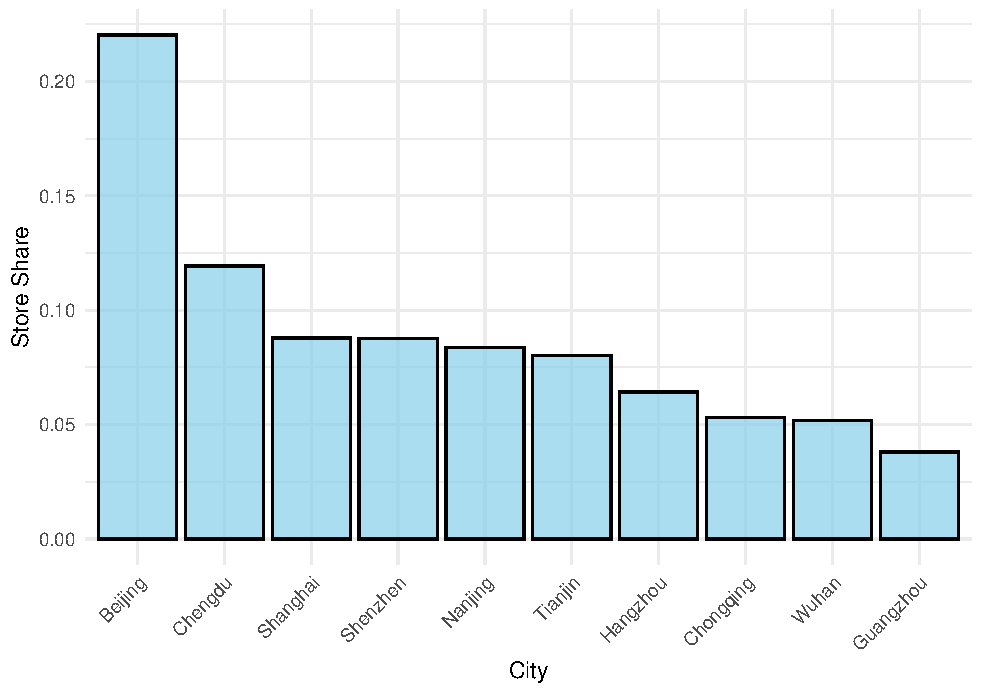
\includegraphics[width=0.7\textwidth]{../figures/distribution_of_ten_cities.pdf}
  \caption{Distribution of Ten Cities's Brokerages Store Shares}
  \label{fig:distribution_store_shares}
  Note: the x-axis is city's name and the y-axis is the offline brokerage's stores share in the city. The data source is from AutoNavi Map.
\end{figure}

% \input{tab_tex/other-regressions.tex}

\begin{figure}[h!]
 \centering
    \begin{minipage}{0.328\textwidth}
        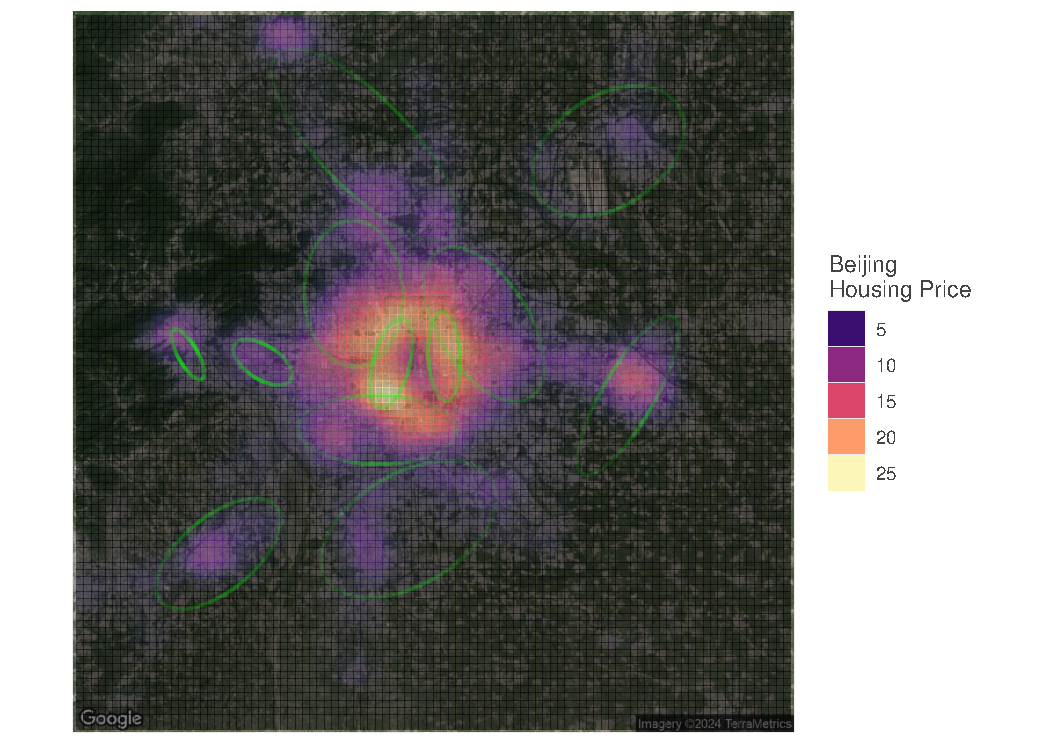
\includegraphics[width=\linewidth]{figures/distribution_of_hp_and_broker/Beijing.pdf}
    \end{minipage}
    \hfill
    \begin{minipage}{0.328\textwidth}
        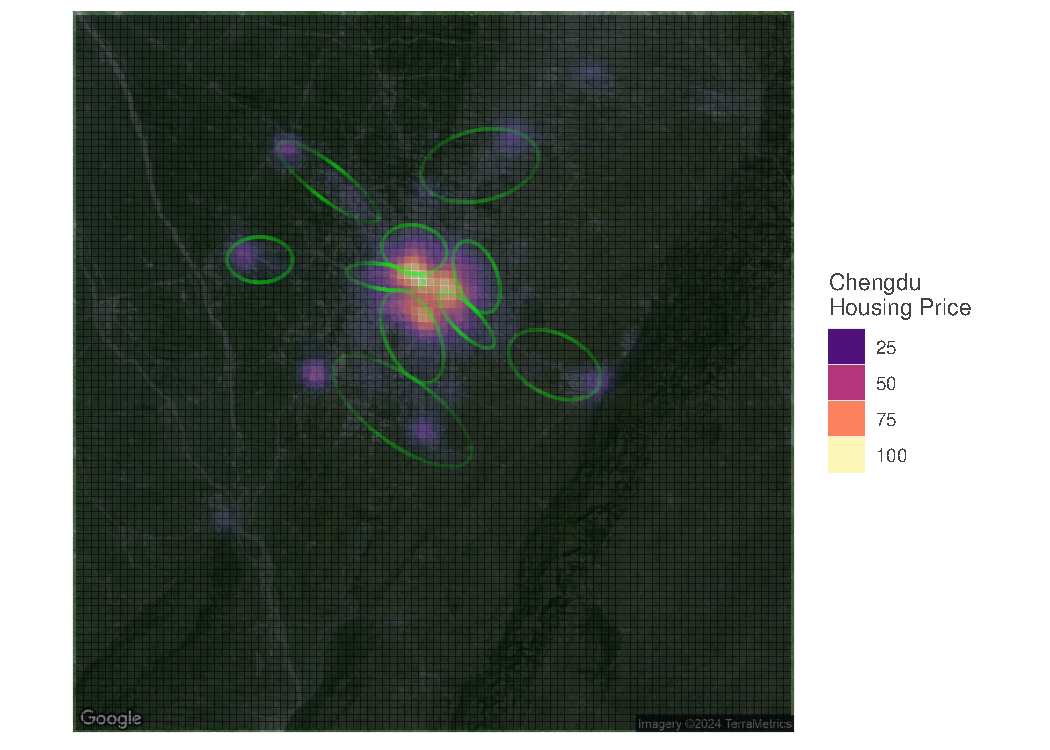
\includegraphics[width=\linewidth]{figures/distribution_of_hp_and_broker/Chengdu.pdf}
    \end{minipage}
    \begin{minipage}{0.328\textwidth}
        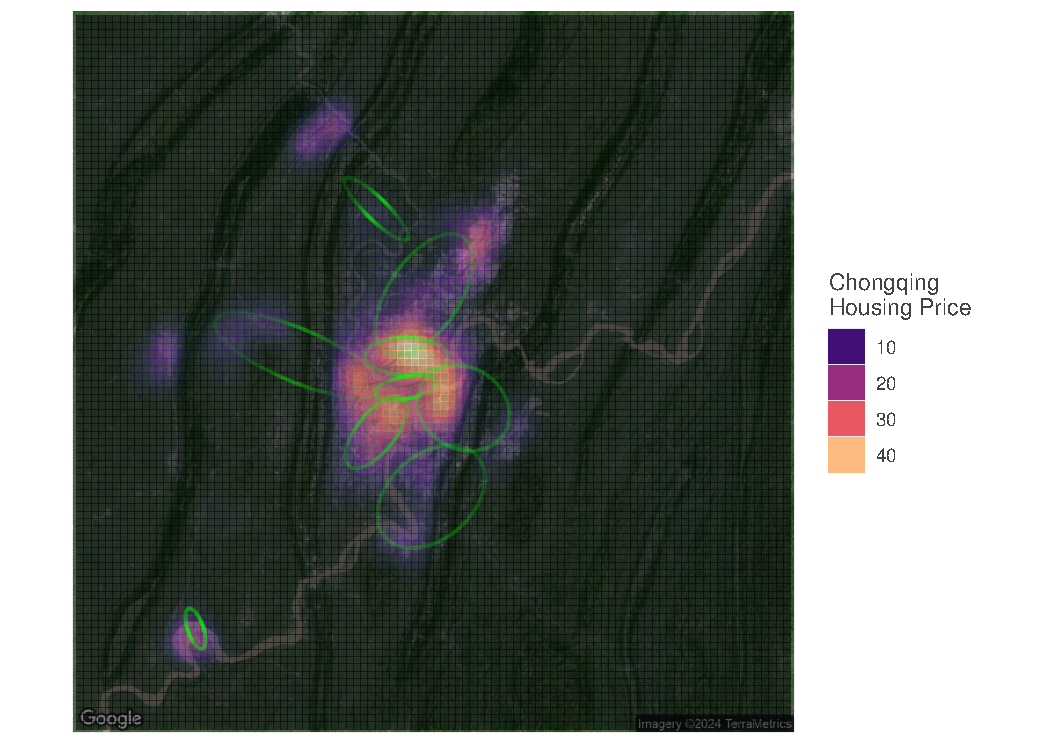
\includegraphics[width=\linewidth]{figures/distribution_of_hp_and_broker/Chongqing.pdf}
    \end{minipage}

    \begin{minipage}{0.328\textwidth}
        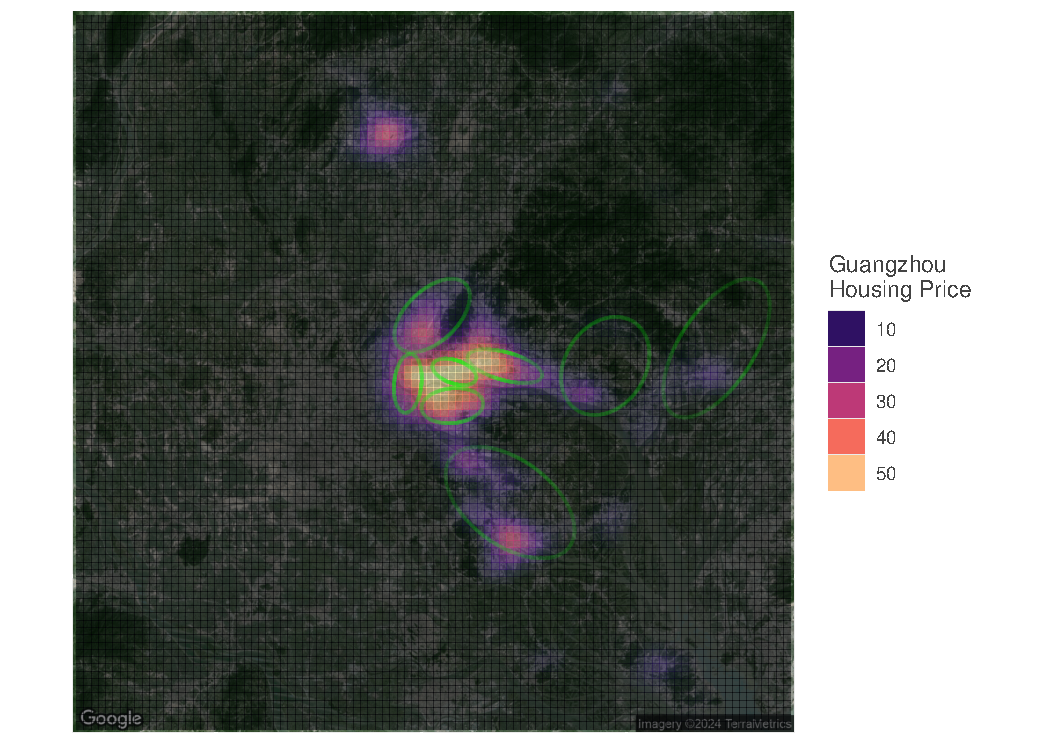
\includegraphics[width=\linewidth]{figures/distribution_of_hp_and_broker/Guangzhou.pdf}
    \end{minipage}
    \hfill
    \begin{minipage}{0.328\textwidth}
        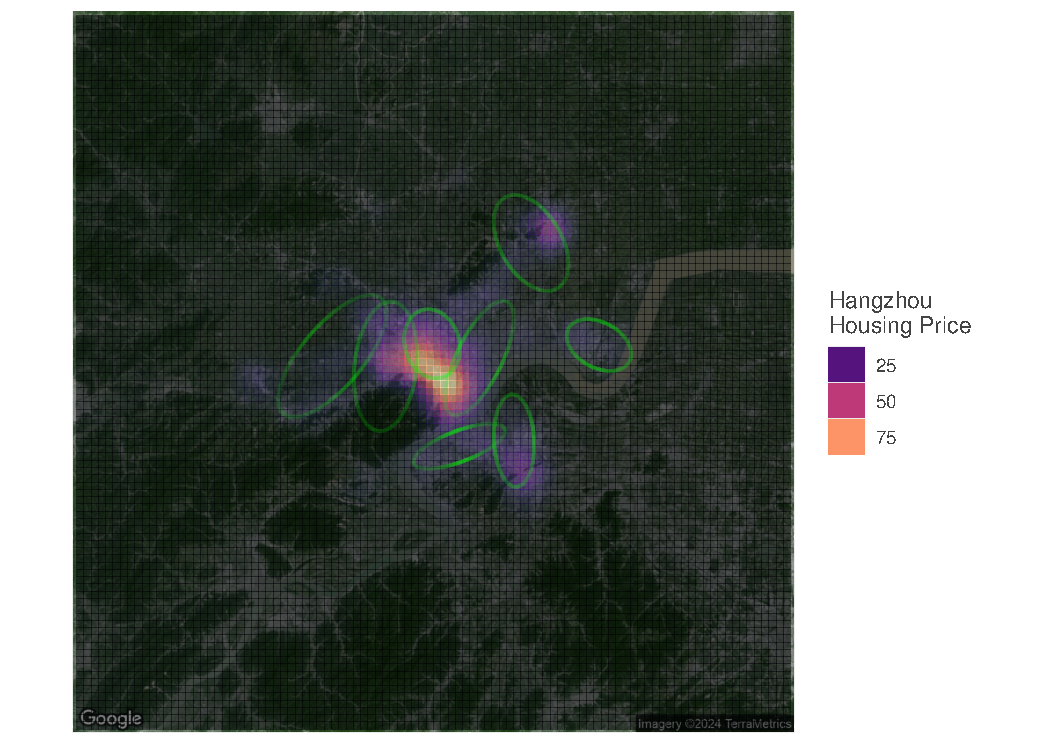
\includegraphics[width=\linewidth]{figures/distribution_of_hp_and_broker/Hangzhou.pdf}
    \end{minipage}
    \begin{minipage}{0.328\textwidth}
        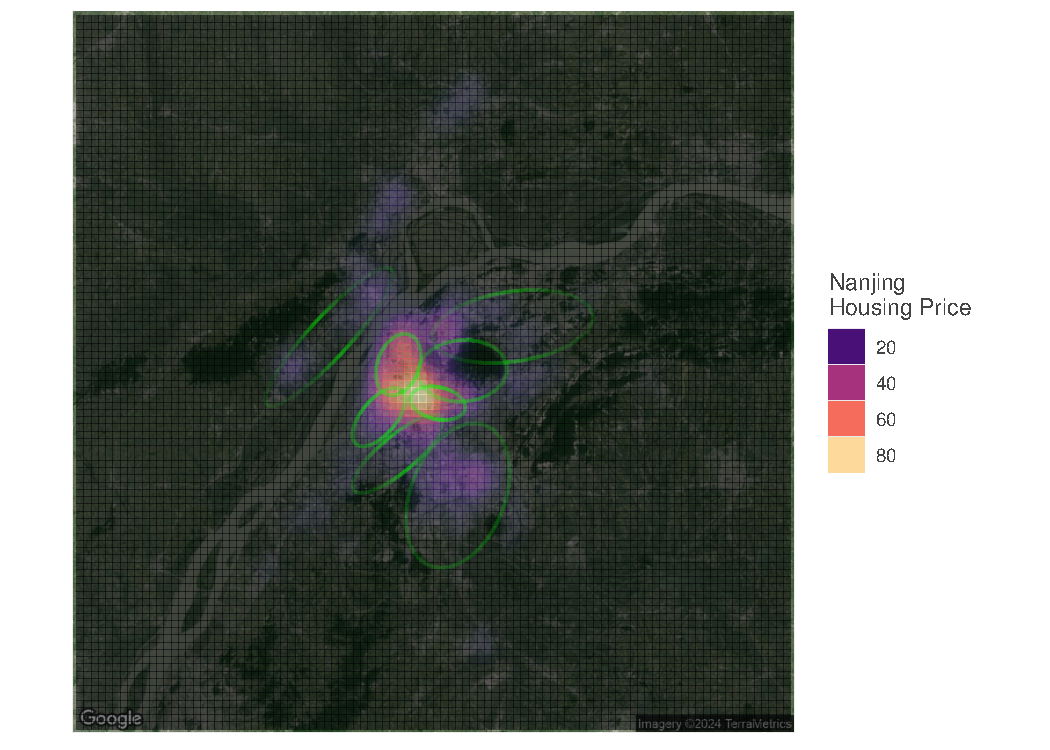
\includegraphics[width=\linewidth]{figures/distribution_of_hp_and_broker/Nanjing.pdf}
    \end{minipage}

    \begin{minipage}{0.328\textwidth}
        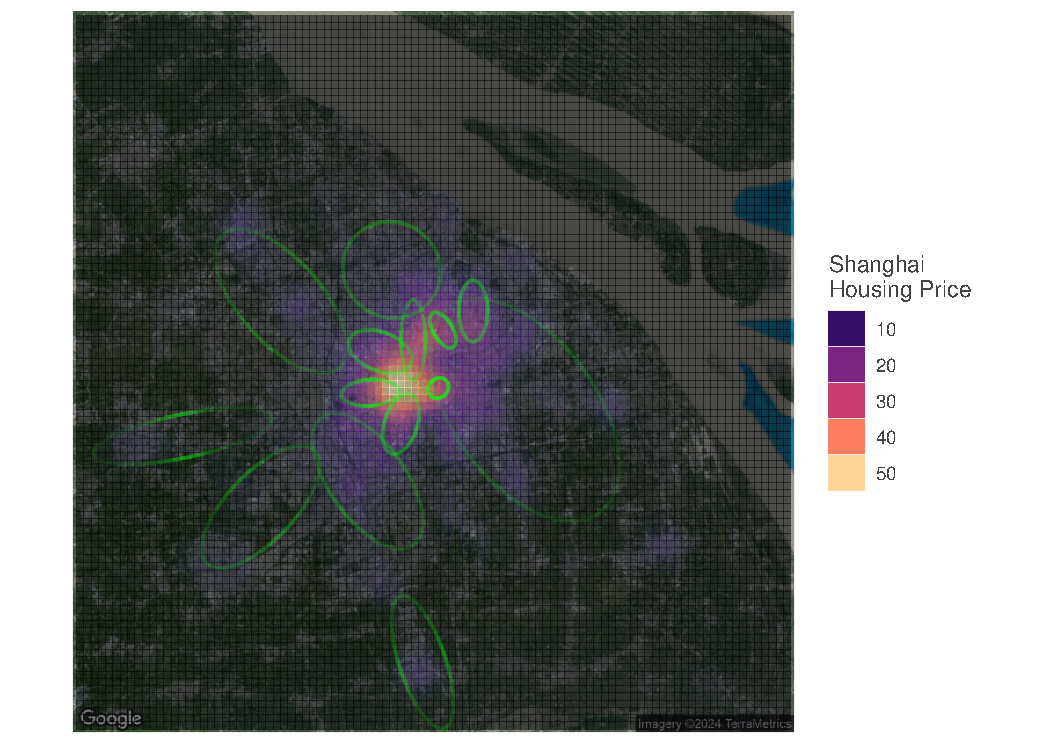
\includegraphics[width=\linewidth]{figures/distribution_of_hp_and_broker/Shanghai.pdf}
    \end{minipage}
    \hfill
    \begin{minipage}{0.328\textwidth}
        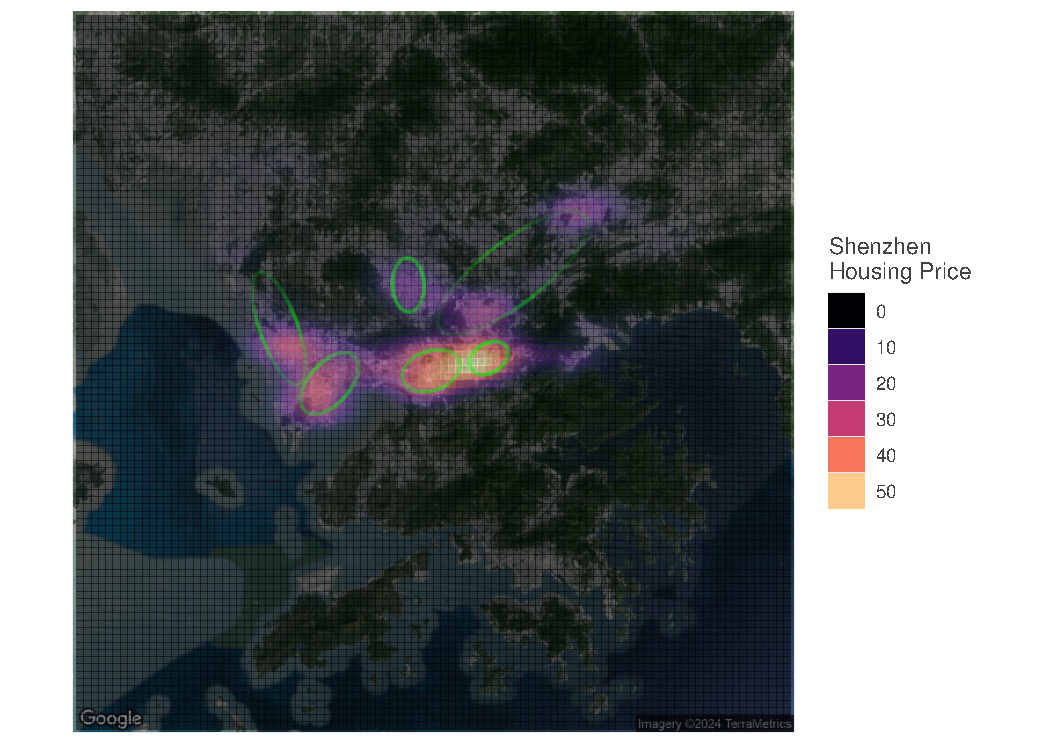
\includegraphics[width=\linewidth]{figures/distribution_of_hp_and_broker/Shenzhen.pdf}
    \end{minipage}
    \begin{minipage}{0.328\textwidth}
        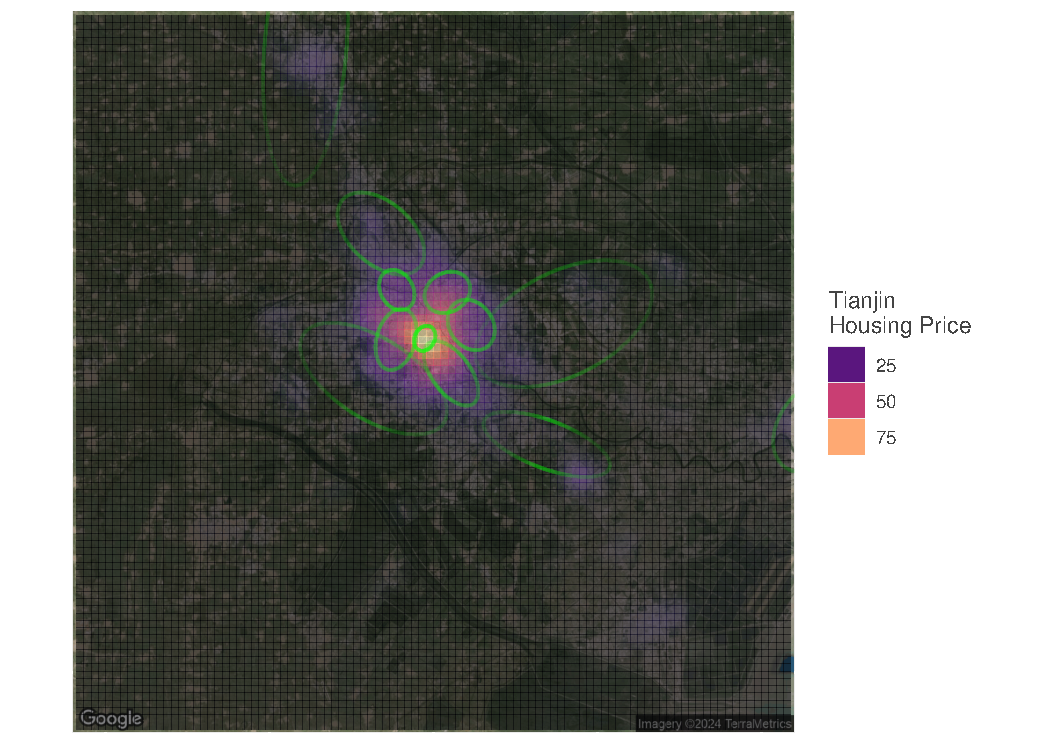
\includegraphics[width=\linewidth]{figures/distribution_of_hp_and_broker/Tianjin.pdf}
    \end{minipage}

    \begin{minipage}{0.328\textwidth}
        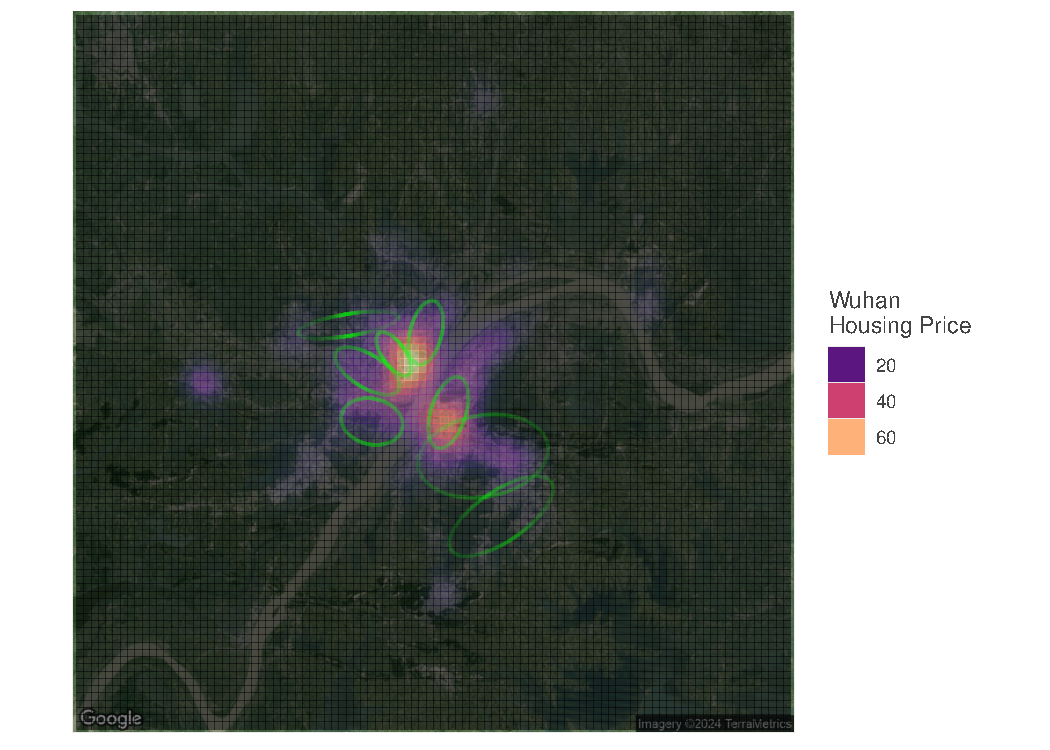
\includegraphics[width=\linewidth]{figures/distribution_of_hp_and_broker/Wuhan.pdf}
    \end{minipage}
    \hfill

\caption{The distribution of housing prices and brokers in different cities}
\label{fig:distribution_of_housing_price_brokers_in_different_cities}

Note: The heat map represents the distribution of housing prices and the standard ellipse represents the distribution of brokers, which is calculated by the mean and standard deviation of the latitude and longitude of brokers. The larger the ellipse, the more sparse the brokerages' distribution is. The Base Map is from Google Map.
 \end{figure}


% latex table generated in R 4.2.0 by xtable 1.8-4 package
% Sun Jun  9 18:04:27 2024
\begin{table}[ht]
\centering
\caption{RD Analysis Donut RD Results with and without Controls} 
\label{tab:rd_robust_results}
\begin{tabular}{llllllll}
  \hline
 &  & \multicolumn{3}{c}{Without Control} & \multicolumn{3}{c}{With Control} \\
Donut Width & Method & Coef & SE & p-value & Coef & SE & p-value \\ 
  \hline
donut\_0.01 & Robust & -0.0527 & 0.0388 & 0.175 & -0.0777 & 0.0522 & 0.136 \\ 
  donut\_0.0125 & Robust & -0.0771 & 0.0434 & 0.076 & -0.11 & 0.0578 & 0.0578 \\ 
  donut\_0.015 & Robust & -0.027 & 0.0485 & 0.578 & -0.113 & 0.0651 & 0.0837 \\ 
  donut\_0.0175 & Robust & -0.0264 & 0.0551 & 0.632 & -0.144 & 0.074 & 0.0517 \\ 
  donut\_0.02 & Robust & 0.0317 & 0.0618 & 0.608 & -0.104 & 0.0836 & 0.214 \\ 
  donut\_0.0225 & Robust & -0.0253 & 0.0708 & 0.721 & -0.115 & 0.0935 & 0.22 \\ 
  donut\_0.025 & Robust & 0.0828 & 0.0806 & 0.304 & 0.0317 & 0.109 & 0.771 \\ 
   \hline
\end{tabular}

Note that the cutoff is 0.41, the main bandwidth is 0.066 and the bias bandwidth is 0.135.
\end{table}



% latex table generated in R 4.2.0 by xtable 1.8-4 package
% Sun Jun  9 18:05:45 2024
\begin{table}[ht]
\centering
\caption{Placebo Test Results for Different Covariates} 
\label{tab:placebo_test_results}
\begin{tabular}{llllllr}
  \hline
Covariate & Estimate & SE & Z & PValue & Bandwidth & EffectiveObs \\ 
  \hline
pop & -73.6 & 396 & -0.186 & 0.852 & 0.066 & 32010 \\ 
  light & -0.203 & 0.26 & -0.779 & 0.436 & 0.066 & 32010 \\ 
  price\_concession & -0.000379 & 0.000739 & -0.513 & 0.608 & 0.066 & 31437 \\ 
  ln\_end\_price & -0.0234 & 0.0167 & -1.41 & 0.16 & 0.066 & 32010 \\ 
  ln\_nego\_changes & -0.000518 & 0.0222 & -0.0233 & 0.981 & 0.066 & 32010 \\ 
  ln\_watch\_time & 0.0726 & 0.0682 & 1.06 & 0.288 & 0.066 & 32010 \\ 
  green\_ratio & -0.00161 & 0.00231 & -0.696 & 0.487 & 0.066 & 32010 \\ 
  bedroom & -0.00858 & 0.0176 & -0.487 & 0.626 & 0.066 & 32010 \\ 
  ln\_watch\_people & 0.0542 & 0.0357 & 1.52 & 0.129 & 0.066 & 32010 \\ 
  living\_room & 0.000998 & 0.0113 & 0.0881 & 0.93 & 0.066 & 32010 \\ 
  ln\_negotiation\_period & -0.00648 & 0.0266 & -0.243 & 0.808 & 0.066 & 32010 \\ 
  museum & -0.0544 & 0.0416 & -1.31 & 0.191 & 0.066 & 32010 \\ 
  kind & 0.00667 & 0.136 & 0.0491 & 0.961 & 0.066 & 32010 \\ 
  mid & 0.0124 & 0.0608 & 0.204 & 0.838 & 0.066 & 32010 \\ 
  sub & 0.046 & 0.0244 & 1.89 & 0.059 & 0.066 & 32010 \\ 
  house\_age & 0.209 & 0.275 & 0.76 & 0.447 & 0.066 & 32010 \\ 
  total\_building & -0.275 & 0.829 & -0.332 & 0.74 & 0.066 & 32010 \\ 
   \hline
\end{tabular}
\end{table}



% latex table generated in R 4.2.0 by xtable 1.8-4 package
% Mon Jul  8 21:20:28 2024
\begin{table}[ht]
\centering
\caption{Placebo Test Results for Different Cutoff Point} 
\label{tab:movement_cutoff}
\begin{tabular}{rlllllr}
  \hline
Cutoff & Estimate & SE & Z & PValue & Bandwidth & EffectiveObs \\ 
  \hline
0.32 & -33154 & 16261 & -2.04 & 0.0415 & 0.0965 & 58710 \\ 
  0.35 & 2112 & 13951 & 0.151 & 0.88 & 0.132 & 75514 \\ 
  0.40 & -25930 & 19778 & -1.31 & 0.19 & 0.0764 & 38332 \\ 
  0.42 & -12532 & 18043 & -0.695 & 0.487 & 0.0855 & 40529 \\ 
  0.45 & -22806 & 17952 & -1.27 & 0.204 & 0.0858 & 36968 \\ 
  0.50 & 25778 & 15534 & 1.66 & 0.097 & 0.133 & 49373 \\ 
  0.65 & 47140 & 21425 & 2.2 & 0.0278 & 0.092 & 20096 \\ 
  0.70 & -32584 & 19286 & -1.69 & 0.0911 & 0.121 & 22549 \\ 
   \hline
\end{tabular}
\end{table}



\clearpage

\begin{table}[H]
  \begin{center}
    \begin{scriptsize}
    \caption{Robustness Check By HHI Index}
    \label{tab:dynamic_hhi}
    {
\def\sym#1{\ifmmode^{#1}\else\(^{#1}\)\fi}
\begin{tabular}{l*{6}{c}}
\toprule
            &\multicolumn{1}{c}{(1)}&\multicolumn{1}{c}{(2)}&\multicolumn{1}{c}{(3)}&\multicolumn{1}{c}{(4)}&\multicolumn{1}{c}{(5)}&\multicolumn{1}{c}{(6)}\\
            &\multicolumn{1}{c}{log(income)}&\multicolumn{1}{c}{log(income)}&\multicolumn{1}{c}{price concession}&\multicolumn{1}{c}{price concession}&\multicolumn{1}{c}{log(lead times)}&\multicolumn{1}{c}{log(lead times)}\\
\midrule
L.ln\_income &     -0.0864\sym{***}&      -0.108\sym{***}&                     &                     &                     &                     \\
            &   (0.00562)         &   (0.00684)         &                     &                     &                     &                     \\
\addlinespace
yearx2\_density&       0.726\sym{***}&       0.136\sym{***}&     0.00260         &    -0.00141         &      0.0300         &      0.0299         \\
            &     (0.110)         &    (0.0438)         &   (0.00446)         &   (0.00156)         &    (0.0847)         &    (0.0317)         \\
\addlinespace
yearx3\_density&       0.430\sym{***}&       0.106\sym{***}&     0.00651         &    -0.00190         &       0.238\sym{***}&      0.0571\sym{*}  \\
            &     (0.113)         &    (0.0396)         &   (0.00397)         &   (0.00149)         &    (0.0849)         &    (0.0297)         \\
\addlinespace
yearx4\_density&       0.281\sym{***}&      0.0229         &     0.00635\sym{*}  &   -0.000630         &       0.163\sym{*}  &      0.0182         \\
            &     (0.103)         &    (0.0399)         &   (0.00363)         &   (0.00143)         &    (0.0850)         &    (0.0303)         \\
\addlinespace
yearx5\_density&       0.220\sym{**} &      0.0420         &    0.000861         &    -0.00108         &       0.215\sym{***}&      0.0531\sym{*}  \\
            &    (0.0976)         &    (0.0418)         &   (0.00324)         &   (0.00136)         &    (0.0716)         &    (0.0304)         \\
\addlinespace
yearx6\_density&      -0.273\sym{**} &      -0.191\sym{***}&    -0.00421         &    -0.00590\sym{**} &      0.0668         &     0.00649         \\
            &     (0.134)         &    (0.0662)         &   (0.00466)         &   (0.00256)         &     (0.102)         &    (0.0480)         \\
\addlinespace
yearx7\_density&      -0.358\sym{***}&      -0.133\sym{*}  &    -0.00135         &    -0.00796\sym{***}&       0.148         &      0.0297         \\
            &     (0.131)         &    (0.0767)         &   (0.00506)         &   (0.00299)         &     (0.112)         &    (0.0604)         \\
\addlinespace
broker\_410  &     0.00129         &     0.00610\sym{*}  &   0.0000350         &   0.0000271         &    0.000518         &     0.00487\sym{**} \\
            &   (0.00128)         &   (0.00342)         & (0.0000461)         &  (0.000137)         &  (0.000952)         &   (0.00246)         \\
\addlinespace
ln\_end\_price&       0.898\sym{***}&       0.966\sym{***}&      0.0651\sym{***}&      0.0787\sym{***}&       0.241\sym{***}&       0.269\sym{***}\\
            &    (0.0366)         &    (0.0591)         &   (0.00248)         &   (0.00387)         &    (0.0294)         &    (0.0434)         \\
\addlinespace
ln\_watch\_people&      0.0605\sym{***}&      0.0636\sym{***}&     0.00194\sym{***}&     0.00153\sym{***}&       0.332\sym{***}&       0.315\sym{***}\\
            &   (0.00473)         &   (0.00666)         &  (0.000208)         &  (0.000272)         &   (0.00530)         &   (0.00676)         \\
\addlinespace
ln\_watch\_time&      0.0303\sym{***}&      0.0308\sym{***}&   -0.000105         &   -0.000319\sym{*}  &      0.0266\sym{***}&      0.0450\sym{***}\\
            &   (0.00300)         &   (0.00409)         &  (0.000123)         &  (0.000174)         &   (0.00263)         &   (0.00342)         \\
\addlinespace
ln\_nego\_changes&      0.0170\sym{**} &      0.0299\sym{**} &     0.00178\sym{***}&     0.00258\sym{***}&       0.134\sym{***}&       0.134\sym{***}\\
            &   (0.00806)         &    (0.0122)         &  (0.000289)         &  (0.000459)         &   (0.00870)         &    (0.0102)         \\
\addlinespace
ln\_negotiation\_period&      0.0606\sym{***}&      0.0575\sym{***}&    -0.00184\sym{***}&    -0.00182\sym{***}&       0.116\sym{***}&       0.143\sym{***}\\
            &   (0.00445)         &   (0.00680)         &  (0.000194)         &  (0.000301)         &   (0.00487)         &   (0.00668)         \\
\addlinespace
L.price\_concession&                     &                     &      -0.183\sym{***}&      -0.205\sym{***}&                     &                     \\
            &                     &                     &   (0.00582)         &   (0.00744)         &                     &                     \\
\addlinespace
L.ln\_lead   &                     &                     &                     &                     &      -0.112\sym{***}&      -0.120\sym{***}\\
            &                     &                     &                     &                     &   (0.00457)         &   (0.00605)         \\
\midrule
\(N\)       &       80476         &       45060         &       77780         &       43578         &       80476         &       45060         \\
R-squared   &       0.892         &       0.908         &       0.638         &       0.699         &       0.925         &       0.929         \\
\bottomrule
\multicolumn{7}{l}{\footnotesize Standard errors in parentheses}\\
\multicolumn{7}{l}{\footnotesize \sym{*} \(p<0.1\), \sym{**} \(p<0.05\), \sym{***} \(p<0.01\)}\\
\end{tabular}
}
  
  
    \end{scriptsize}
  \end{center}
\end{table}

\clearpage

% \begin{table}[H]
%   \begin{center}
%     \begin{scriptsize}
%     \caption{Robustness Check By Market Maturity Index}
%     \label{tab:platform_consolidation_hetero_mature}
%     {
\def\sym#1{\ifmmode^{#1}\else\(^{#1}\)\fi}
\begin{tabular}{l*{4}{c}}
\toprule
            &\multicolumn{1}{c}{(1)}&\multicolumn{1}{c}{(2)}&\multicolumn{1}{c}{(3)}&\multicolumn{1}{c}{(4)}\\
            &\multicolumn{1}{c}{log(income) [lower]}&\multicolumn{1}{c}{log(income) [higher]}&\multicolumn{1}{c}{log(lead times) [lower]}&\multicolumn{1}{c}{log(lead times) [higher]}\\
\midrule
L.ln\_income &     -0.0529\sym{***}&     -0.0929\sym{***}&                     &                     \\
            &   (0.00594)         &   (0.00539)         &                     &                     \\
\addlinespace
yearx2\_density&       0.197\sym{***}&      0.0979\sym{*}  &      0.0260         &      0.0582         \\
            &    (0.0586)         &    (0.0502)         &    (0.0406)         &    (0.0373)         \\
\addlinespace
yearx3\_density&       0.207\sym{***}&      0.0242         &       0.129\sym{***}&      0.0224         \\
            &    (0.0483)         &    (0.0463)         &    (0.0345)         &    (0.0373)         \\
\addlinespace
yearx4\_density&       0.114\sym{**} &     -0.0313         &      0.0540\sym{*}  &      0.0282         \\
            &    (0.0453)         &    (0.0440)         &    (0.0318)         &    (0.0326)         \\
\addlinespace
yearx5\_density&       0.128\sym{***}&      0.0437         &      0.0250         &      0.0647\sym{*}  \\
            &    (0.0423)         &    (0.0492)         &    (0.0315)         &    (0.0330)         \\
\addlinespace
yearx6\_density&     -0.0765         &      -0.237\sym{***}&      0.0139         &     -0.0107         \\
            &    (0.0814)         &    (0.0805)         &    (0.0493)         &    (0.0565)         \\
\addlinespace
yearx7\_density&      -0.116         &      -0.103         &     -0.0161         &      0.0817         \\
            &    (0.0883)         &    (0.0872)         &    (0.0724)         &    (0.0774)         \\
\addlinespace
broker\_410  &     0.00416\sym{***}&   -0.000302         &    0.000511         &    0.000930         \\
            &   (0.00155)         &   (0.00142)         &   (0.00114)         &   (0.00110)         \\
\addlinespace
ln\_end\_price&       0.945\sym{***}&       0.928\sym{***}&       0.233\sym{***}&       0.255\sym{***}\\
            &    (0.0429)         &    (0.0409)         &    (0.0326)         &    (0.0322)         \\
\addlinespace
ln\_watch\_people&      0.0863\sym{***}&      0.0501\sym{***}&       0.327\sym{***}&       0.331\sym{***}\\
            &   (0.00529)         &   (0.00505)         &   (0.00550)         &   (0.00564)         \\
\addlinespace
ln\_watch\_time&      0.0282\sym{***}&      0.0327\sym{***}&      0.0309\sym{***}&      0.0334\sym{***}\\
            &   (0.00392)         &   (0.00310)         &   (0.00295)         &   (0.00276)         \\
\addlinespace
ln\_nego\_changes&      0.0259\sym{***}&      0.0200\sym{**} &       0.160\sym{***}&       0.110\sym{***}\\
            &   (0.00911)         &   (0.00886)         &   (0.00812)         &   (0.00901)         \\
\addlinespace
ln\_negotiation\_period&      0.0488\sym{***}&      0.0657\sym{***}&       0.123\sym{***}&       0.129\sym{***}\\
            &   (0.00517)         &   (0.00487)         &   (0.00487)         &   (0.00534)         \\
\addlinespace
L.ln\_lead   &                     &                     &     -0.0922\sym{***}&      -0.107\sym{***}\\
            &                     &                     &   (0.00461)         &   (0.00496)         \\
\midrule
\(N\)       &       66143         &       67756         &       66143         &       67756         \\
R-squared   &       0.883         &       0.897         &       0.917         &       0.927         \\
\bottomrule
\multicolumn{5}{l}{\footnotesize Standard errors in parentheses}\\
\multicolumn{5}{l}{\footnotesize \sym{*} \(p<0.1\), \sym{**} \(p<0.05\), \sym{***} \(p<0.01\)}\\
\end{tabular}
}
  
  
%     \end{scriptsize}
%   \end{center}
% \end{table}

\begin{figure}
    \centering
    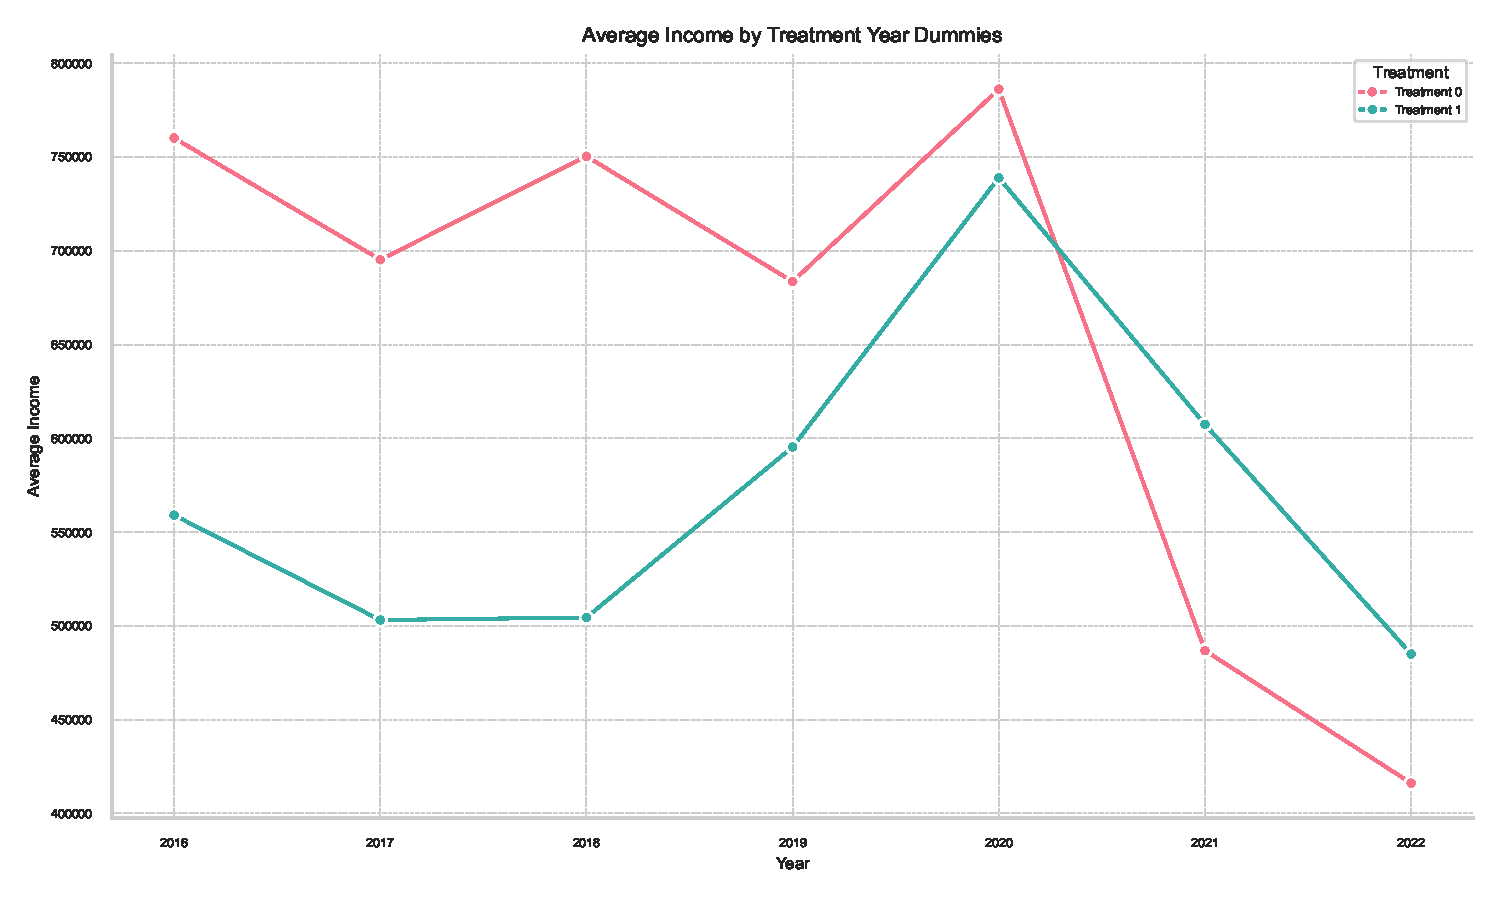
\includegraphics[width=0.7\textwidth]{../figures/average_income_by_treatment_platform.pdf}
    \caption{Treatment Effect of platform consolidation}
    \label{fig:treatment_consolidation}
    Note: the x-axis is year and the y-axis is the average income of Lianjia in each year. The graph uses the neighborhood-level data.
\end{figure}

\begin{table}[H]
  \begin{center}
    \begin{scriptsize}
    \caption{Codebook}
    \label{tab:codebook}
    \begin{tabular}{lll}
\toprule
Name & Label & Dimension \\
\midrule
income & The income lianjia in this given district/housing. & $10^5 \times$ \textyen \\
lead\_times & The time it takes before a deal is made. & counts \\
price\_concession & price changes (ending price - starting price) / starting price & \% \\
density & percentage of lianjia to all brokerages & \% / 100 \\
broker\_410 & number of other brokerages within 410 meters, which is the cutoff of RD & counts \\
watching\_people & The number of people watching this listing. & counts \\
end\_price & The final agreed price. & \textyen \\
non\_online\_effect & without online platformization influence & bool indicator \\
watched\_times & The number of times a listing is watched. & counts \\
nego\_times & The number of times a negotiation was held. & counts \\
nego\_period & The period over which negotiations took place. & days \\
jiadian & Referring to electronic shops. & counts \\
kind & Referring to proximity to kindergartens & counts \\
hotel & Referring to proximity to hotels & counts \\
shop\_mall & Referring to shopping mall. & counts \\
museum & Distance to the nearest museum. & counts \\
old & Referring to old care systems. & counts \\
ktv & Referring to KTV and some entertainment venues. & counts \\
mid & Referring to middle schools. & counts \\
prim & Referring to primary schools. & counts \\
west\_food & Referring to the availability of western food nearby. & counts \\
super & Referring to proximity to supermarkets (measured by number within given distance & counts \\
sub & Referring to proximity to subway stations. & counts \\
park & Referring to parks. & counts \\
area & The area of a property. & $m^2$ \\
bedroom & The number of bedrooms in a property. & counts \\
toilet & The number of toilets in a property. & counts \\
house\_age & The age of the house. & years \\
floor\_level & The level on which a particular room or apartment is, within a building. & categories \\
green\_ratio & The ratio of the green space to the total plot area. & \% / 100 \\
total\_building & The total number of buildings in an area. & counts \\
total\_floor\_number & The number of floors in a building. & counts \\
living\_room & The number of living rooms in a property. & counts \\
elevator\_ratio & The ratio of elevators to the total number of floors. & \% / 100 \\
kitchen & The number of kitchens in a property. & counts \\
floor\_ratio & The ratio of the floor area to the total plot area. & fraction \\
total\_resident & The total number of residents in an area. & counts \\
pm25 & Air quality measure. & mass/volume \\
pop & Population density. & people/$km^2$ \\
light & Night time lights. & lux \\
\bottomrule
\end{tabular}
  
  
    \end{scriptsize}
  \end{center}
\end{table}





\end{document}
